\documentclass[french]{report}
\usepackage[T1]{fontenc}
\usepackage[utf8]{inputenc}
\usepackage[francais]{babel}
\usepackage{eurosym}
\usepackage{verbatim}
%~ \usepackage{color}
\usepackage{fancyhdr} %the perpage package
\usepackage{multirow}
\usepackage{framed}
\usepackage[dvipsnames]{xcolor}
\usepackage[colorlinks = true,
            linkcolor = DarkOrchid,
            urlcolor  = BlueViolet,
            citecolor = MidnightBlue,
            anchorcolor = ForestGreen]{hyperref}
\usepackage{graphicx}
\usepackage[margin=3.3cm]{geometry}
\usepackage{caption}
\usepackage{enumitem}
\usepackage{amsmath}
\usepackage{amssymb}
\usepackage{array}
\usepackage{listings}
\lstset{
  basicstyle=\ttfamily,
  columns=fullflexible,
  %frame=single,
  breaklines=true,
  postbreak=\mbox{\textcolor{red}{$\hookrightarrow$}\space},
}
\DeclareMathOperator{\atantwo}{atan2}

\setlength\parindent{0pt} %noindent pour tout le document

\newcommand{\revoir}[1]{\textcolor{OrangeRed}{#1}}
\usepackage{hyperref}

\newcommand{\textfoot}{Comp3d v5 : fondements mathématiques}

\pagestyle{fancyplain}
\fancyhf{}
 \renewcommand{\headrulewidth}{0pt}
 \renewcommand{\footrulewidth}{1pt}
\rhead{ \fancyplain{}{} }
\lhead{ \fancyplain{}{} }
\lfoot{ \fancyplain{}{\textfoot} }
\rfoot{ \fancyplain{}{\thepage} }

\makeatletter
\renewcommand*\env@matrix[1][\arraystretch]{%
  \edef\arraystretch{#1}%
  \hskip -\arraycolsep
  \let\@ifnextchar\new@ifnextchar
  \array{*\c@MaxMatrixCols c}}
\makeatother


\begin{document}

\renewcommand{\labelitemi}{$\bullet$}

	\begin{tabular*}{\textwidth}{l p{10cm} l}
		\multirow{8}{*}{\includegraphics[width=3cm]{images/logo_ign}} & \centering \begin{small} \textbf{{Institut national de l'information géographique et forestière}} \end{small} & \\

																																			 & \centering \begin{small}\textbf{SGM-ENSG}\end{small}& \\
																																			 %& \centering \begin{small} {SBV/PBL}\end{small}
                                                                       & &\\ \cline{2-3}

																																			& \centering \begin{small}JM Muller \end{small} &\\
																																			&	\centering \begin{small}2024 \end{small}&

	\end{tabular*}

\vspace{1.5cm}

\begin{framed}
	\centering
		\vspace{0.5cm}

		\textbf{\LARGE{Comp3d version 5 : fondements mathématiques}}

		\vspace{0.5cm}
\end{framed}




%\maketitle
\newpage

\tableofcontents

\chapter*{Introduction}
\addcontentsline{toc}{chapter}{Introduction}
\pagenumbering{arabic}

Le programme de compensation de micro-géodésie Comp3D permet de calculer des réseaux peu étendus
(quelques kilomètres) avec compensation simultanée en bloc des observations planimétriques et altimétriques.
Il est particulièrement bien adapté pour les réseaux de surveillance, et plus précisément la
détermination de coordonnées et la détection de mouvements.
Il a été développé par le Docteur Yves EGELS, de l'IGN (Institut Géographique National) et est actuellement maintenu par JM Muller (IGN/ENSG).


Ce document présente l'utilisation des moindres carrés dans l'ajustement de réseaux géodésiques.
Il décrit les algorithmes et les formules utilisées par Comp3D. Il permet aussi d'améliorer son
utilisation et l'interprétation des résultats.


\chapter{Systèmes de coordonnées}
\section{Géoréférencement}

Comp3D travaille en interne dans un repère local tridimentionnel (cf. \ref{systlocal}).

On peut toutefois utiliser une projection géoréférencée en entrée et en sortie.
Pour cela Comp3D utilise la bibliothèque proj (\url{http://proj.org/}) pour passer de
coordonnées dans une projection quelconque à la projection stéréographique locale décrite en \ref{systlocal}.

Il est à noter que les $\sigma$ a priori et a posteriori sur les points et les azimuts sont toujours exprimés dans
le repère local de Comp3D (cf. \ref{spheriques}).
Ils ne sont donc pas entâchés de l'altération linéaire et de la convergence des méridiens de la projection d'entrée.

Seules les coordonnées des points sont données dans la projection choisie par l'utilisateur
et converties par Comp3D dans le repère local de calcul pour le calcul (cf. \ref{systlocal}).

En cas de géoréférencement, le centre du chantier est exprimé dans le repère géoréférencé.
Il sert à la fois à calculer la latitude centrale
du chantier et à définir le point de tangence (et l'origine) de la projection stéréographique locale.


\section{Système local tridimensionnel}\label{systlocal}

Tout le calcul est effectué dans un repère local tridimensionnel.

Les coordonnées en entrée (fichier COR) et en sortie (fichier NEW) sont données en projection stéréographique oblique si on est en mode local, ou dans une projection choisie par l'utilisateur. Dans ce dernier cas, les coordonnées sont passées dans une projection stéréographique oblique.

La projection stéréographique oblique est définie par son point tangent qui est aussi le centre du chantier.

Les points sont donnés au départ avec :
\begin{itemize}
\item leurs coordonnées plani ($E$ et $N$)
\item leur coordonnée alti ($h$)
\end{itemize}

Le système local est défini par la sphère tangente à l'ellipsoïde au centre du chantier.
%~ L'ellipsoïde de référence est \textbf{International-Hayford 1909} défini par :
%~ \begin{itemize}
%~ \item demi grand axe : $a = 6378388.0000m$
%~ \item excentricité : $e = 0.081991889979$
%~ \end{itemize}
L'ellipsoïde de référence est \textbf{GRS80} :
\begin{itemize}
\item demi grand axe : $a = 6378137.0000m$
\item excentricité au carré : $e^2 = 0.00669438$
\end{itemize}

%\begin{figure}[h]
\begin{center}
\includegraphics[width = 10cm]{images/sphere_courbure_totale}
%\caption{}
\end{center}
%\end{figure}

Le rayon de la sphère est égal à la courbure totale de l'ellipsoïde au point de tangence :
$$R_S = a \frac{ \sqrt {1-e^2} }{1-e^2 \sin ^2 {\phi} }$$




On définit les points suivants :
\begin{itemize}
\item $O$ est le centre de la sphère. $O$ est aussi l'origine du système 3D
\item $A$ est le barycentre du réseau
\item $B$ est le pôle opposé de $A$
\item $I$ est un point du système local à transformer dans le système 3D
\item $h$ est sa hauteur
\item $I'$ est le point projeté sur le plan tangent, il est associé à $I$
\item $J'$ est le point de la sphère, résultant de la transformation stéréographique oblique inverse de $I'$
\item $J$ est le point final, il est donné dans le système 3D
\end{itemize}

%\begin{figure}[h]
\begin{center}
\includegraphics[width = 10cm]{images/coupe}
%\caption{}
\end{center}
%\end{figure}

A partir des coordonnées horizontales ($E$ et $N$) définissant le point $I'$, il est possible de déterminer
les coordonnées du point associé sur la sphere ($J'$).
Ensuite la coordonnée verticale $h$ est supposée donnée dans la direction de la normale à la sphère.
En effet, le géoïde est localement approximé par cette sphère.

Les paramètres $X_{centre}$, $Y_{centre}$ et $\mu$ peuvent être utilisés de façon à pouvoir imiter localement n'importe quelle projection conforme
(tant que l'altération linéaire ne varie pas trop dans le chantier, étant donné que $\mu$ est constante)
car pour une zone assez petite toutes les projections sont équivalentes au premier ordre.


\begin{center}
$\left\{
  \begin{array}{c}
    X_{spher} = \frac{E_{stereo}-E_{centre}}{\mu \alpha} \\[0.3cm]
    Y_{spher} = \frac{N_{stereo}-N_{centre}}{\mu \alpha} \\[0.3cm]
    Z_{spher} = H_{COR}
  \end{array}
\right.
\qquad
$ où
$\qquad
\alpha = 1+ \frac{((X_{COR}-X_{centre})/\mu) ^2 + ((Y_{COR}-Y_{centre})/\mu) ^2}{ 4 R_S ^2}
$
\end{center}

%On peut par exemple utiliser des coordonnées Lambert 93 en donnant l'altération linéaire au centre du chantier (et en vérifiant que ses variations sont
%négligeables sur l'emprise du chantier par rapport à la précision recherchée), et en prenant pour coordonnées du centre les coordonnées Lambert 93
%du centre du chantier.

La coordonnée verticale des points en entrée doit être proche de la hauteur ellipsoïdale réelle, étant donné que cela a une grande influence sur l'échelle planimétrique (voir \ref{spheriques}).


\section{Coordonnées sphériques}\label{spheriques}

Comp3D fonctionne en coordonnées sphériques, ce qui a pour avantage d'avoir en tout point un axe $Z$ qui suit la verticale locale (en supposant que le géoïde suit
localement la sphère de courbure totale), comme le font les appareils de mesures qui sont bullés.

L'échelle planimétrique est choisie pour que à $Z = 0$, une unité planimétrique corresponde à 1m :

\begin{center}
\includegraphics[width = 10cm]{images/coord_spher}
\end{center}

On voit qu'avec ces coordonnées on ne peut pas calculer la distance entre deux points par la formule classique :
$$d_{AB} = \sqrt{(X_A-X_B)^2+(Y_A-Y_B)^2+(Z_A-Z_B)^2}$$


Il faut passer par l'angle
au centre de la Terre ($\alpha$). La formule utilisée est :
$$ d_{AB}  = \sqrt{(Z_A-Z_B)^2+4 . Z_A .Z_B . (\sin(\alpha/2))^2} $$

Par contre, cela simplifie certaines observations telles que des dénivellées :
$$ \Delta_{H_{AB}}  = (Z_B-Z_A) $$

C'est aussi le cas pour tous les types d'observations où la verticale est prise en compte.

\section{Fonctions utilisées en coordonnées sphériques}

Angle au centre de la Terre entre les points A et B :
$$\alpha=  \sqrt{ \left(\frac{X_B-X_A}{R}\right)^2 + \left(\frac{Y_B-Y_A}{R}\right)^2 }$$
Implémenté dans la fonction
\texttt{arc()}
qui donne $C_{AB} = \cos(\alpha)$  et $S_{AB} = \sin(\alpha)$.

Azimut $az$ entre deux points A et B (connaissant $C_{AB}=\cos(\alpha)$) :
$$ az = \atantwo(X_B-C_{AB}.X_A,Y_B.Z_A'-Y_A.Z_B')$$
où $$ Z_A' = \sqrt{1-\left(\frac{X_A}{R}\right)^2-\left(\frac{Y_A}{R}\right)^2}$$
et $$ Z_B' = \sqrt{1-\left(\frac{X_B}{R}\right)^2-\left(\frac{Y_B}{R}\right)^2}$$

Implémenté dans \texttt{azimuth()}.

\section{Coordonnées cartésiennes}\label{cartesiennes}

Or il arrive que la direction de la gravité ne nous intéresse pas, et des coordonnées cartésiennes locales sont plus utiles.

Dans ce cas l'axe Z est toujours parallèle à une verticale arbitraire.

On peut alors travailler plus simplement avec des coordonnées 3D, ce qui est particulièrement utile quand on mélange différentes
sources (scanner 3D, résultats de calculs photogrammétriques etc.).

\begin{center}
\includegraphics[width = 8cm]{images/coord_cart}
\end{center}

On voit qu'avec ces coordonnées on peut calculer la distance entre deux points par la formule classique :
$$d_{AB} = \sqrt{(X_A-X_B)^2+(Y_A-Y_B)^2+(Z_A-Z_B)^2}$$

Comp3D exporte les coordonnées compensées en cartésiennes (fichier 3D), de façon à ce que les résultats soient facilement
interprétables par des logiciels fonctionnant en coordonnées cartésiennes.

Ce type de coordonnées est aussi utilisé pour la compensation des observations de type bascule (voir \ref{bascule}).

L'intérêt des repères cartésiens est qu'une simple application matricielle permet de passer de l'un à l'autre.


\newpage

\section{Liste des repères de Comp3D}

\begin{center}
\includegraphics[width = 14cm]{images/frames}
\end{center}

\begin{itemize}
\item \textbf{projection d'entrée} (non représentée), celle du fichier .cor quand on est géoréférencé, qui est convertie en projection stéréographique locale, ou projection stéréographique locale si non géoréférencé.
\item \textbf{repère sphérique} du chantier (en vert), proche de la projection stéréographique locale, celui dans lequel sont les paramètres des moindres carrés correspondants aux coordonnées des points, son origine est au point central du chantier (ici $O$). L'axe Z suit la normale à la sphère d'approximation. L'axe Y suit la direction du Nord géographique à l'origine du repère, il y a donc une rotation entre ce repère et celui de la projection d'entrée correspondant à la convergence des méridiens de ce dernier.
\item \textbf{repère cartésien géocentrique} (non représenté), intermédiaire de calcul pour passer au repère cartésien global. N'a de sens que si le projet est géoréférencé.
\item \textbf{repère cartésien global} du chantier (en bleu), dont les axes coincident avec cuex du repère sphérique au point d'origine et dont l'origine est confondue avec celle du repère sphérique.
\item \textbf{repère cartésien vertical} en un point (en magenta), qui coincide avec le repère sphérique en ce point (à la déviation de la verticale près), son origine est sur le point (hors hauteur de station). Z est donc la direction de la normale au géoïde sur le point.
\item \textbf{repère cartésien local instrument} en un point (en jaune), repère propre d'un instrument qui n'est pas forcément bullé, son origine est sur le point (hors hauteur de station).
\end{itemize}



\section{De sphériques à cartésiennes}

\begin{center}
\includegraphics[width = 8cm]{images/coord_spher_cart}
\end{center}

En vert on a les coordonnées sphériques de 4 points, et en rouge leurs coordonnées cartésiennes.
Ici la verticale fixée pour les coordonnées sphériques est celle du point \texttt{vert\_ref\_spher} en sphériques.

Pour passer des coordonnées sphériques aux coordonnées cartésiennes, on retourne à la projection stéréoscopique,
puis on passe aux cartésiennes géocentriques avec libproj et on fait une transformation rigide pour passer aux
coordonnées cartésiennes dans le repère global du chantier.

Pour avoir une idée du facteur d'échelle entre les deux méthodes de calcul de distance
(c'est à dire si on confond coordonnées sphériques et cartésiennes), il suffit de faire le calcul :
$$ echelle = (R + z) / R $$
avec R rayon de la Terre, et z la hauteur (ellipsoïdale) du chantier.
Exemple : à 100m de hauteur : $echelle = (6400+0.1)/6400 \approx 1.000015$ soit 15ppm.




\section{Approximation entre repères sphérique et cartésien}

Comp3D travaille dans son repère "sphérique", mais effectue un calcul rigoureux
pour les sous-repères cartésiens (.xyz) : il fait les conversions nécessaires pour
que les observations des sous-repères soient bien prises en compte.

Dans le cas de chantiers de lidar terrestre où on a à recaler des gros nuages
de points, il pourrait être intéressant de proposer une transformation matricielle
(plus facilement optimisable) pour passer au mieux du repère cartésien d'un instrument
au repère en projection d'entrée (.cor).

Ce calcul serait approximatif, mais suffisant si les stations ne visent pas trop
loin et que la précision n'est pas trop importante.


\subsection{Exemple}
Soient deux stations mesurant des cibles dans leur sous-repère cartésien :
\begin{center}
\includegraphics[width = 9cm]{images/ex_approx_spher_xyz_local}
\end{center}

Avec la station $St1$ placée au centre du chantier ($St1=O$) et bullée ($\overrightarrow{Oz} \| \overrightarrow{h}$),
on a pour résultat :

\begin{center}
\includegraphics[width = 11cm]{images/ex_approx_spher_xyz_global}
\end{center}
En rouge on retrouve les repères cartésiens locaux des stations, en bleu les coordonnées dans le repère cartésien global, et vert celles dans le repère sphérique.
On voit que les coodonnées diffèrent de façon non linéaire quand on s'éloigne de l'origine du chantier.

La station $St2$ a son $z$ local aligné avec celui des coordonnées cartésiennes globales. Sa rotation pour passer
du repère cartésiens local au global est donc l'identitée. Par contre la station $St2$ n'est pas bullée : son $z$
n'est pas perpendiculaire à la sphère.

Comp3D fournit les transformations à 6 paramètres pour passer rigoureusement des repère cartésiens locaux
des instruments au repère cartésien global du chantier dans les fichier .xyz :

\begin{verbatim}
Extrait de St1.xyz :

**!  Station    : St1
*  S =               0.0000 0.0000 0.0000
*              1.000000        0.000000       -0.000000
*  R =        -0.000000        1.000000        0.000000
*              0.000000        0.000000        1.000000
****  instr = R.(global-S) <=> global = R'.instr +S  ****
\end{verbatim}

\begin{verbatim}
Extrait de St2.xyz :

**!  Station    : St2
*  S =            2000.0000 0.0000 -0.0000
*              1.000000        0.000000       -0.000000
*  R =        -0.000000        1.000000        0.000000
*              0.000000       -0.000000        1.000000
****  instr = R.(global-S) <=> global = R'.instr +S  ****
\end{verbatim}

Si on applique ces transformations aux mesures des instruments,
on obtient les coordonnées cartésiennes globales du chantier.
Celles-ci sont très différentes des coordonnées sphériques ou en projection d'entrée,
mais elles ont l'intérêt de coincider parfaitement.

On cherche ici une meilleure transformation pour pouvoir travailler en coordonnées
de la projection d'entrée et minimiser les erreurs.

Ce qu'on veut faire, "redresser" les coordonnées sphériques pour rendre le repère cartésien :
\begin{center}
\includegraphics[width = 8cm]{images/ex_approx_spher_xyz_spher_redress}
\end{center}

On cherche ensuite la meilleure transformation matricielle entre les repère cartésiens locaux
des instruments et ce repère.
\begin{center}
\includegraphics[width = 8cm]{images/ex_approx_spher_xyz_spher_redress2}
\end{center}

Le niveau d'erreur dépend de la distance de visée dans les sous-repères,
de leur éloigement au centre du chantier, de l'altération linéaire et
de la hauteur ellipsoïdale.

%~ Si on reprend le même exemple, mais avec la station $St1$ placée en hauteur :

%~ \begin{center}
%~ \includegraphics[width = 11cm]{images/ex_approx_spher_xyz_global_h}
%~ \end{center}

%~ \begin{center}
%~ \includegraphics[width = 8cm]{images/ex_approx_spher_xyz_spher_redress_h}
%~ \end{center}

%~ On voit que les mesures des instruments semblent trop grandes par rapport aux coordonnées.

%~ On peut alors remettre à l'échelle la composante planimétrique des mesures d'un facteur
%~ $\rho/(\rho+h)$ :

%~ \begin{center}
%~ \includegraphics[width = 8cm]{images/ex_approx_spher_xyz_spher_redress_h2}
%~ \end{center}

\subsection{Formules}


\subsubsection{Transformation}
La transformation matricielle est donnée par :

$$
 P_{proj} = R_{\gamma} \cdot S_{proj} \cdot S_h \cdot R_{cart2spher}^\top \cdot R^\top \cdot P_{instr} + T
$$

Où :

\begin{itemize}
  \item  $T$ : coordonnées compensées de la station dans le repère utilisateur (fichier .new).
  \item  $P_{instr}$ : le point dans le repère catésien de l'instrument
  \item  $R_{cart2spher}$ : la matrice de rotation correspondant au "redressement" des coordonnées sphériques (voir plus bas)
  \item  $R$ : rotation entre le repère cartésien global et celui de l'instrument. C'est la matrice donnée dans le fichier .xyz.
  \item  $S_h$ : la matrice de mise à l'échelle liée à la hauteur de l'instrument (avec $\rho$ le rayon de la sphère) :
$$S_h=\begin{pmatrix}[1.5]
\rho/(\rho+h) & 0 &  0 \\
0 & \rho/(\rho+h) & 0 \\
 0 &  0 & 1 \\
\end{pmatrix}$$

  \item  $S_{proj}$ : la matrice de mise à l'échelle liée au module linéaire de la projection ($\mu$) :
$$S_{proj}=\begin{pmatrix}[1.5]
\mu & 0 &  0 \\
0 & \mu & 0 \\
 0 &  0 & 1 \\
 \end{pmatrix}$$
  \item $R_{\gamma}$ : rotation correspondant à la convergence des méridiens à l'origine du chantier :
$$R_{\gamma}=\begin{pmatrix}[1.5]
\cos{\gamma} & -\sin{\gamma} &  0 \\
\sin{\gamma} & \cos{\gamma} & 0 \\
 0 &  0 & 1 \\
\end{pmatrix}$$


\end{itemize}



\subsubsection{Rotation entre cartésiennes et sphériques}


La correction de rotation due au "redressement" des coordonnées sphériques
est la pente de la courbe correspondant à l'image de l'axe $Z = constante$
en coordonnées sphériques.

Voici l'image d'une grille cartésienne $1km \times 1km$ en coordonnées sphériques (abscisse: $E$, ordonnée : $h$, en km) :
\begin{center}
\includegraphics[width = 15cm]{images/cartgrid_in_spherical}
\end{center}


On cherche à exprimer $h$ en fonction de $E$. Pour le point $P$ (coordonnées cartésiennes globales $(X,Z)$,
coordonnées sphériques $(E, h)$), $M$ le projeté central de $P$ sur la sphère et $\alpha$ l'angle au centre de la Terre $C$ :

\begin{center}
\includegraphics[width = 8cm]{images/ex_approx_spher_xyz_h_vs_E}
\end{center}


on a :
 %~ $$ \overrightarrow{CO} =
 %~ \begin{pmatrix}[1.5]
%~ 0 \\
%~ \rho \\
%~ \end{pmatrix} $$
 $$ E = \mu \cdot \rho \cdot \alpha $$
 $$ \overrightarrow{CP} =
 \begin{pmatrix}[1.5]
X \\
Z + \rho \\
\end{pmatrix} $$
 $$ \overrightarrow{CM} =
 \begin{pmatrix}[1.5]
\rho \cdot \sin{\alpha} \\
\rho \cdot \cos{\alpha} \\
\end{pmatrix} $$
 $$ \frac{\rho+h}{\rho} \cdot \overrightarrow{CM} = \overrightarrow{CP} $$

D'où
$$\left\{
    \begin{array}{ll}
        \left(\rho+h\right) \cdot \sin{\alpha} = X  \\
        \left(\rho+h\right) \cdot \cos{\alpha} = Z + \rho 
\end{array}
\right.$$

%~ $$\left\{
    %~ \begin{array}{ll}
        %~ \tan{\alpha} = \frac{X}{Z + \rho}  \\
        %~ \rho+h = \frac{Z + \rho}{\cos{\alpha}}
%~ \end{array}
%~ \right.$$

$$\left\{
    \begin{array}{ll}
        \alpha = \arctan{\frac{X}{Z + \rho}}  \\
        h = \frac{Z + \rho}{\cos{\alpha}} - \rho
\end{array}
\right.$$

On obtient donc la formule de $h$ en fonction de $E$ :
$$ h(E) = \frac{Z + \rho}{\cos{\frac{E}{\mu \rho}}} - \rho $$


Et sa dérivée :

 $$ \frac{\partial h(E)}{\partial E} = \frac{ \frac{Z+\rho}{\mu \rho} \cdot \sin\frac{E}{\mu \rho}}{\cos^2\frac{E}{\mu \rho}} $$

On a donc à faire une rotation de :

 $$ \beta = \arctan \frac{\partial h(E)}{\partial E} $$
 $$ \beta = \arctan  \left(\frac{ \frac{Z+\rho}{\mu \rho} \cdot \sin\frac{E}{\mu \rho}}{\cos^2\frac{E}{\mu \rho}}\right) $$
 
À la fois pour la composante $E$ et la composante $N$ pour obtenir la matrice $R_{cart2spher}$
(via la fonction $angEN2Rot\_small\_angles()$).


\subsubsection{Application}


Dans le cas décrit plus haut ($St2$ à $1000m$ du centre, faisant des visées de $1000m$ vers le centre
et vers l'opposé), on a des résidus de $8cm$ en $h$ pour tous les points, alors que la différence
de coordonnées sphériques est de $70cm$ vers l'extérieur.
Le fait que les résidus soient les mêmes dans les deux directions montre que la rotation appliquée
est optimale.


\section{Coordonnées cartésiennes géocentriques}

Le passage entre coordonnées cartésiennes locales ($P_{cl}$) et cartésiennes géocentriques ($P_{cg}$) est fait par une transformation rigide à 6 paramètres.

$$P_{cg} = R . P_{cl}  + T$$

\begin{center}
\includegraphics[width = 10cm]{images/cart_geocentr}
\end{center}

La latitude et la longitude de l'origine du chantier ainsi que les coordonnées du point origine du repère local en cartésiennes géocentriques ($=T$) sont calculées par libproj.

La partie rotation $R$ correspond au passage de Est-Nord-Haut (xyz) vers XYZ géocentrique. Il s'agit simplement de tourner de la longitude et de la latitude :
en partant du repère local, il faut tourner de $-lon$ autour de l'axe des $Z$, puis de $\pi/2-lat$ autour de l'axe des $Y$.
On se retrouve alors avec un repère au pôle nord, pour lequel il faut encore faire une rotation de $\pi/2$ autour de l'axe $Z$.

Ce qui donne en équations :

$$Rz=\begin{pmatrix}[1.5]  cos(lon) & sin(lon)&  0 \\ -sin(lon) & cos(lon) & 0 \\  0 &  0 & 1 \\ \end{pmatrix}$$
$$Ry=\begin{pmatrix}[1.5] cos(pi/2-lat) & 0 & -sin(pi/2-lat) \\  0 & 1 & 0 \\ sin(pi/2-lat) & 0 & cos(pi/2-lat) \\ \end{pmatrix}$$
$$Rz2=\begin{pmatrix}[1.5] 0 & 1 & 0 \\ -1 & 0 & 0 \\ 0 & 0 & 1 \\ \end{pmatrix}$$
$$R=(Rz2.Ry.Rz)^\top$$

Pour créer un fichier Sinex il faut exporter les coordonnées compensées et la matrice de variance-covariance en coordonnées cartésiennes géocentriques.

La matrice de variance-covariance de Comp3D est calculée en coordonnées sphériques locales. On commence par supposer que la matrice est
pratiquement la même en coordonnées cartésiennes locales \revoir{(impact ?)}.

Soit $Q_{xx,local}$ la matrice de variance-covariance des coordonnées des points en coordonnées locales.
Il ne s'agit pas directement de celle exportée par Comp3D vu que tous les paramètres hors des coordonnées des points sont enlevés, et qu'on ajoute
des lignes et des colonnes pour les coordonnées qui ne sont pas des paramètres (pour les points 1D et 2D). La matrice a donc une taille de $(3n x 3n)$ avec $n$ le nombre de points.

$$Q_{XX,local}=\begin{pmatrix}[1.5]
	 q_{x1,x1} &  q_{x1,y1} & q_{x1,z1} & \dots & q_{x1,xn} & q_{x1,yn} & q_{x1,zn} \\
	  \vdots   &  \vdots   &  \vdots   &  \vdots   &  \vdots   &  \vdots   &  \vdots \\
     q_{zn,x1} &  q_{zn,y1} & q_{zn,z1} & \dots & q_{zn,xn} & q_{zn,yn} & q_{zn,zn} \\ \end{pmatrix}$$

Comme on a la formule de passage des coordonnées cartésiennes locales aux cartésiennes géocentriques $P_{cg} = R . P_{cl}  + T$,
on peut faire une propagation de la variance, déjà pour le point $i$ :

$$Q_{XX,geocentr,pt_i} = R . Q_{XX,local,pt_i} . R^{\top}$$

Pour pouvoir appliquer ça à un ensemble de points, on passe par la matrice $R_{total}$ :

$$R_{total}=\begin{pmatrix}[1.5]
    R & 0 & \dots & \dots  & 0 \\
    0 & R & 0 &  & \vdots \\
    \vdots & 0 & \ddots & \ddots & \vdots \\
    \vdots &  & \ddots & \ddots & 0 \\
     0 & \dots &  \dots & 0 & R \\ \end{pmatrix}$$

On obtient alors la matrice de variance-covariance en coordonnées cartésiennes géocentriques :

$$Q_{XX,gecentr} = R_{total} . Q_{XX,local} . R_{total}^{\top}$$

\section{Gestion des repères via libproj}

En entrée du processus on a la définition de la projection utilisateur \texttt{projDef}, qui vaut par exemple
\texttt{"IGNF:LAMB93"} pour travailler en Lambert 93 et les coordonnées planimétriques du centre du chantier \texttt{c\_user} (dont le $h$ vaut $0$) dans cette même projection.

On calcule les coordonnées géographiques du centre du chantier \texttt{c\_geogr} en utilisant la définition \texttt{"+proj=latlong"} :

\begin{verbatim}
defLatLong = "+proj=latlong"
pj_in2latlong = proj_create_crs_to_crs(0, projDef, defLatLong, 0)
c_geogr = proj_trans(pj_in2latlong, PJ_FWD, c_user)
\end{verbatim}

On a donc la latitude du centre du chantier, qui sert à trouver le rayon de la sphère locale.

Cette transformation est également utilisée pour donner les coordonnées géographiques des points initiaux et finaux pour l'affichage sur le plan leaflet du rapport.

Et on fabrique la matrice de rotation entre le repère cartésien global du chantier et le repère cartésien géocentrique \texttt{RotGlobal2Geocentric} :

\begin{verbatim}
c_longitude = c_geogr.x * PI/180
c_latitude  = c_geogr.y * PI/180

Rz <<  cos(c_longitude), sin(c_longitude), 0,
      -sin(c_longitude), cos(c_longitude), 0,
                      0,                0, 1

Ry<< cos(PI/2 - c_latitude), 0,  -sin(PI/2 - c_latitude),
                          0, 1,                        0,
     sin(PI/2 - c_latitude), 0,   cos(PI/2 - c_latitude)

Rz2<< 0,  1,  0,
     -1,  0,  0,
      0,  0,  1

RotGlobal2Geocentric = (Rz2*Ry*Rz).transpose()
\end{verbatim}

On calcule ensuite les coordonnées du centre du chantier en coordonnées cartésiennes géocentriques \texttt{c\_geocent} :

\begin{verbatim}
defGeocentr = "+proj=geocent"
pj_in2geocent = proj_create_crs_to_crs(0, projDef, defGeocentr, 0)
c_geocent = proj_trans(pj_in2geocent, PJ_FWD, c_user)
\end{verbatim}

Avec \texttt{RotGlobal2Geocentric} et \texttt{c\_geocent}, la fonction de passage entre repère cartésien global du chantier et le repère cartésien géocentrique est complète :

$$ P_{geocent} = R_{global2geocent} \times P_{cart\_global} + C_{geocent}$$

On peut maintenant créer la définition de la projection stéréographique locale \texttt{stereo\_def}, pour se mettre dans le même état que pour un calcul non géoréférencé :

\begin{verbatim}
stereo_def = "+proj=sterea +lat_0=[c_geogr.y] +lon_0=[c_geogr.x] +k_0=1 +x_0=0 +y_0=0"
pj_in2stereo = proj_create_crs_to_crs(0, projDef, stereo_def, 0)
\end{verbatim}

Cette transformation sera utilisée pour convertir les coordonnées lues dans le fichier cor :

\begin{verbatim}
p_stereo = proj_trans(pj_in2stereo, PJ_FWD, p_cor)
\end{verbatim}

Et la transformation inverse est utilisée pour convertir les coordonnées CAP et compensées dans la projection utilisateur.

\begin{verbatim}
p_new = proj_trans(pj_in2stereo, PJ_INV, p_compense)
\end{verbatim}

Dans le cas d'un calcul non-géoréférencé, le processus est le même,
en déclarant pour définition de la projection d'entrée \texttt{projDef} :

\begin{verbatim}
projDef = "+proj=sterea +lat_0=[latitude] +lon_0=0 +k_0=1 +x_0=[c_user.x] +y_0=[c_user.y]"
\end{verbatim}

De cette manière on peut passer des coordonnées locales aux géographiques ou cartésiennes géocentriques,
même si le géoréférencement n'a pas de sens, simplement en intermédiaire pour obtenir des différences de
coordonnées géographiques ou des coordonnées cartésiennes locales.

Résumé des passages entre repères :

\begin{center}
\includegraphics[width = 14cm]{images/all_frames}
\end{center}

\newpage

\section{Gestion des coordonnées sphériques et cartésiennes pour observations cartésiennes}

Les paramètres des moindres carrés sont les coordonnées sphériques des points.
Cela est parfaitement adapté aux mesures topométriques, mais pour des observations
type ajustement de sous-repère cartésien ou de ligne de base GNSS, il faut passer par les coordonnées cartésiennes.

Prenons un exemple simplifié, où on a une seule observation, $\Delta_X = 99$ (en coordonnées cartésiennes dans le repère lié au point $A$), entre les points $A$ et $B$. On prend ici un rayon terrestre très petit pour exagérer les erreurs.

Les coordonnées sphériques (en vert, avec pour axes $E$ et $h$) ont pour origine le point $O$, le centre du chantier.

On travaille ici avec le repère cartésien "vertical" lié au point $A$ (en bleu, avec pour axes $X$ et $Z$).
Celui-ci a pour origine $A$ et pour orientation de repère sphérique au point $A$. L'axe $Z$ est aligné avec l'axe vertical au point $A$.

\begin{center}
\includegraphics[width = 12cm]{images/cart_spher_obs}
\end{center}

Les paramètres des moindres carrés sont donc $(E_A, h_A)$ et $(E_B, h_B)$.
Pour chaque point on peut calculer ses coordonnées dans n'importe quel repère cartésien.
Ici, on va nommer $(X_A, Z_A)$ et $(X_B, Z_B)$ les coordonnées des points dans le repère cartésien vertical lié au point A. Par définition, $(X_A, Z_A) = (0, 0)$.

L'observation qu'on a ici est donc :

$$\dot{X_B} - \dot{X_A} = 99m$$

On peut imaginer que c'est une observation faite avec un scanner laser bullé, centré en $A$.

Avec nos coordonnées approchées, on trouve :

$$X_B - X_A = 100m$$

On a donc un résidu de $1m$ sur cette observation. On remarque que si on néglige la différence entre coordonnées cartésiennes et sphériques, on trouve un résidu de $E_B - E_A = 9m$. Il est donc indispensable de calculer le résidu à partir des coordonnées cartésiennes.

La jacobienne de l'observation est :

$$\begin{pmatrix}[1.5] \frac{\partial \Delta_X}{\partial X_A}\\ \frac{\partial \Delta_X}{\partial X_B} \end{pmatrix}
=\begin{pmatrix}[1.5] -1\\ 1 \end{pmatrix}$$

Après compensation on devrait ainsi trouver $(\hat{X_A}, \hat{h_A}) = (0.5, 0)$ et $(\hat{X_B}, \hat{h_B}) = (99.5, 0)$ en l'absence d'autres contraintes.

Le problème est que $X_A$ et $X_B$ ne sont pas les paramètres des moindres carrés.

Les coordonnées sphériques compensées correspondantes seraient
$(\hat{E_A}, \hat{h_A}) = (0.5, 0.01)$ et $(\hat{E_B}, \hat{h_B}) = (139.6, 19.7)$

On voit donc que cette observation qui ne touche que $X_A$ et $X_B$ modifie aussi $h_A$ et $h_B$.

\ \\

Si on fait l'approximation $\partial X_B = \partial E_B$ (comme c'est le cas jusqu'à Comp3D version 5.20),
cette observation ne touchera pas $h_A$ et $h_B$. On compte sur une éventuelle observation $\Delta_Z$ pour modifier $h_A$ et $h_B$. Le fait de calculer les résidus à partir des coordonnées cartésiennes devrait itérativement devrait nous approcher de la valeur compensée correcte.

Si cette solution n'est pas parfaite elle peut être suffisante pour des mesures de portée courte ($<100m$) comme c'est le cas pour les mesures scanner et tracker. Pour les lignes de bases GNSS, la portée peut être beaucoup plus grande et donc la différence entre $\partial X_A$ et $\partial E_A$ non négligeable.

On va donc chercher à exprimer correctement la jacobienne dans le repère sphérique (ici $v$ représente le résidu de l'observation, la direction dans laquelle elle tire les points) :
\begin{center}
\includegraphics[width = 12cm]{images/cart_spher_obs_res}
\end{center}

Comme le repère cartésien où l'observation est exprimée est vertical au point A, on a bien $\partial X_A = \partial E_A$ et $\partial Z_A = \partial h_A$. Cela signifie que $h_A$ ne sera pas modifié par cette observation, mais cela est dû à la linéarisation, et sera corrigé à l'itération suivante.

$$
\begin{pmatrix}[1.5] \frac{\partial \Delta_X}{\partial E_A}\\ \frac{\partial \Delta_X}{\partial h_A}\end{pmatrix}
=
\begin{pmatrix}[1.5] \frac{\partial \Delta_X}{\partial X_A}\\ \frac{\partial \Delta_X}{\partial Z_A} \end{pmatrix}
=
\begin{pmatrix}[1.5] -1\\ 0 \end{pmatrix}
$$


Localement, entre le repère cartésien et le repère sphérique au niveau du point B, on a une simple rotation d'angle $\alpha$, l'angle au centre de la Terre entre $A$ et $B$ plus la différence de déviation de la verticale.



$$
\begin{pmatrix}[1.5] \frac{\partial \Delta_X}{\partial E_B}\\ \frac{\partial \Delta_X}{\partial h_B}\end{pmatrix}
=
\begin{pmatrix}[1.5] \cos(\alpha) & -\sin(\alpha) \\ \sin(\alpha) & \cos(\alpha) \end{pmatrix}
.
\begin{pmatrix}[1.5] \frac{\partial \Delta_X}{\partial X_B}\\ \frac{\partial \Delta_X}{\partial Z_B} \end{pmatrix}
=
\begin{pmatrix}[1.5] \cos(\alpha) & -\sin(\alpha) \\ \sin(\alpha) & \cos(\alpha) \end{pmatrix}
.
\begin{pmatrix}[1.5] 1\\ 0 \end{pmatrix}
$$

On a maintenant tous les éléments pour ajouter cette observation dans la matrice $A$ des moindres carrés, sans autre approximation que la linéarisation.

En pratique, la rotation est de $0.5^o$ pour une ligne de base de 55km, et les résultats finaux ne présentent pas de différence avec l'approche des versions <5.20.
\ \\

Pour ce qui est de la variance (et éventuelles covariances) de l'observation, si celles-ci sont déjà exprimées dans le repère cartésien vertical en $A$, il n'y a rien à faire, car toute l'équation d'observation est toujours dans ce repère.

\section{Coordonnées approchées}

Chaque point a des coordonnées approchées. Elles sont utilisées pour linéariser le problème.
En effet l'ajustement par moindres carrés a besoin d'équations d'observation linéaires, et les
nôtres ne le sont pas. Pour obtenir la solution des moindres carrés, les coordonnées sont
recalculées à chaque itération jusqu'à ce qu'elles satisfassent à la condition de moindre
somme des carrés des résidus.

Comp3d version 5 peut calculer automatiquement les coordonnées approchées de points qui n'ont pas été
définis dans le fichier COR.
Si un point est déclaré dans le fichier COR, les coordonnées données sont utilisées comme point de
départ pour les moindres carrés. Elles doivent donc être suffisamment proches de la réalité pour
que le calcul puisse converger.




\section{Points de référence et précision}
Un point est une référence lorsque ses coordonnées sont contraintes, que ce soit pour leurs trois coordonnées ou simplement la partie planimétrique ou altimétrique. Ces points ajoutent des contraintes à l'ajustement. Les coordonnées contraintes sont associées à des précisions, données par $(\sigma_x,\sigma_y,\sigma_z)$ dans le fichier .COR.

La précision est utilisée pour donner le poids de l'équation de contrainte. Un point bien connu (grande précision) a plus d'influence dans la compensation qu'un autre moins précis.

Toutes ces contraintes sont exprimées dans le repère sphérique, qui n'est pas affecté de l'éventuelle altération linéaire ou convergence des méridiens de la projection d'entrée.



\chapter{Modèle mathématique des moindres carrés}
\section{Modèle fonctionnel}
Le modèle fonctionnel est l'ensemble des relations entre les éléments, qu'ils aient été mesurés ou pas. En général, si les éléments qui ont été mesurés sont
représentés par un vecteur $l$ (m,1), et ceux qui ne l'ont pas été mais dont les valeurs doivent être estimées par moindres carrés sont représentés par $x$ (u,1).
Les $c$ relations fonctionnelles peuvent être exprimées par $f(x,l)=0$,
où $f$ représente les $c$ fonctions $f_i$. Les vecteurs $x$ et $l$ représentent les éléments, pas leurs valeurs estimées ou mesurées.
Cette équation est le modèle fonctionnel pour les éléments $x$ et $l$.
Un modèle fonctionnel peut être incomplet. Cela se produit quand il est impossible de déterminer $x$ fonction de $l$ ou inversement.

\section{Modèle stochastique}
Le modèle stochastique exprime la nature stochastique de la mesure de $l$. Il est habituel de définir une matrice de poids $P$.

Dans le cas où les mesures sont indépendantes, $P$ est diagonale. Le poids d'une observation est proportionnel à l'inverse de l'erreur standard.
Le facteur d'échelle est unique pour tout l'ajustement et est appelé variance \textit{a priori}.
Un modèle stochastique peut être faux si le poids d'une observation n'est pas cohérent avec le reste.

Comme les mesures ne sont pas toujours indépendances (par exemple dans le cas des lignes de base GNSS), on remplit une matrice de variance-covariance des observations $Q$, et on en déduit $P=Q^{-1}$.

Tous les $\sigma^2$ sont divisés par la constante $WEIGHT\_FACTOR = 0.0000001 \approx 0.0003^2$, pour que les valeurs diagonales soient proches de $1$.
Ce facteur est à appliquer sur les variances en sortie.

\section{Paramètres}
Dans l'ajustement par moindres carrés, les paramètres sont les inconnues, c'est à dire les coordonnées des points à déterminer. Ces paramètres doivent d'abord être approximés, pour pouvoir linéariser le problème. Un processus itératif amène alors à une estimation de plus en plus fine des coordonnées.


\section{Linéarisation et itération}
La linéarisation du modèle fonctionnel (en n'utilisant que les termes d'ordres 0 et 1 du développement de Taylor) est utilisée pour permettre d'obtenir
une solution numérique pour les paramètres et les mesures corrigées estimées par les moindres carrés.
Ce n'est valide que parce que les termes d'ordre deux et plus sont insignifiants. C'est pour cela que de bonnes valeurs initiales sont nécessaires.
D'un autre côté, la valeur des paramètres à estimer est rarement assez précise au premier calcul, et on doit effectuer un calcul itératif.
Supposons un ensemble de valeurs de départ $x_0$. On les utilise pour calculer les matrices et on obtient les valeurs $x_1$ à ajouter aux valeurs initiales.
On utilise ensuite les paramètres plus précis $(x_0 + x_1)$ comme nouvelle valeur initiale et on répète la procédure autant de fois qu'il est nécessaire pour arriver au moment où tous les éléments d'une solution $x_i$ sont insignifiants.

L'estimation finale des moindres carrés est $\hat{x}=x_0 + x_1 + x_2 + \dots + x_i$.

Les corrections des valeurs mesurées sont maintenant calculées.
Pendant les itérations, les valeurs des observations ne sont pas modifiées en calculant les corrections après chaque itération.


\section{Formulaire}

Une fois tous les points et les stations définis, une liste des paramètres est créée.
Chaque paramètre a son rang dans le système. On appelle $X$ le vecteur des paramètres.

Chaque observation ajoute une ligne aux matrices $A$ et $P$ et au vecteur $B$.
Le vecteur $B$ contient la partie constante des observations (le résidu).
Dans $A$ on ajoute les dérivées partielles de l'observation suivant chacun des paramètres (numéro de colonne = rang du paramètre).
$P$ est toujours (pour l'instant) une matrice diagonale contenant les $\frac{1}{\sigma_{obs_i}^2}$.

On appelle $ N = A^T P A $ la matrice normale du système.

Une itération de calcul revient à résoudre le système $ A \delta X = B $ par moindres carrés avec les poids $P$.
Pour cela il n'est pas nécessaire de calculer $ N^{-1} $, on utilise ici
\textbf{SparseQR} de la bibliothèque \textbf{Eigen}.

On change ensuite les paramètres : $$ X \leftarrow X + \delta X$$
et on passe à l'itération suivante.

En fin de calcul on peut calculer l'inverse de la matrice normale pour avoir la variance des paramètres :
$$ Q_{\hat{x}\hat{x}} = N^{-1} $$

Et en déduire la matrice de variance/covariance des observations :
$$ Q_{\hat{l}\hat{l}} = A . Q_{\hat{x}\hat{x}} . A^T $$



\chapter{Equations d'observation}



Soit $A(X_A,Y_A,Z_A)$ la station d'où on mesure et $B(X_B,Y_B,Z_B)$ le point visé.
Ces coordonnées viennent des données dans le repère sphérique (voir \ref{spheriques}),
avec
$$Z_A = h_A + R_S + h_{station}$$
$$Z_B = h_B + R_S + h_{cible}$$
avec $R_S$ le rayon de la sphère d'approximation.

L'angle au centre de la sphère $O$ entre $A$ et $B$ est
défini par son sinus $S_{AB}$ et son cosinus $C_{AB}$.

La distance réduite au niveau zéro de l'observation est donc :
$$ D_{0,AB} = R_S . \arcsin(S_{AB})$$
la distance horizontale au niveau de la station est :
$$ D_{hz,AB} = Z_A . \arcsin(S_{AB})$$
 et la distance spatiale est :
$$D_{AB} = \sqrt{(Z_A-Z_B)^2+4 Z_A Z_B \sin^2 \left( \frac{\arcsin(S_{AB})}{2} \right) }$$

La valeur de la mesure est notée $l$.


\section{Poids des observations}

La précision \textit{a priori} d'une observation ($\sigma_{total}$) est calculée en fonction
des précisions entrées par l'utilisateur ($\sigma_{abs}$ et $\sigma_{rel}$) et de la distance $D_{AB}$.

La formule utilisée dépend du type de mesure :
\begin{itemize}
 \item pour contraintes de coordonnés, la formule est : $\sigma_{total} = \sigma_{abs}$
 \item pour mesures homogènes à une distance, la formule est : $\sigma_{total} = \sigma_{abs} + \sigma_{rel} . D_{AB}$
 \item pour mesures homogènes à un angle, la formule est : $\sigma_{total} = \sigma_{abs} + \sigma_{rel} / D_{AB}$ 
\end{itemize}

\section{Dénivellée}
Si la dénivellée entre A et B est mesurée, le modèle fonctionnel est :
$$f(x,l) = Z_B - Z_A - l \quad \text{où} \quad x=
\begin{pmatrix}[1.5] Z_A\\ Z_B \end{pmatrix}$$

Cette équation est linéaire.

La matrice jacobienne est :

$$\begin{pmatrix}[1.5] \frac{\partial f}{\partial Z_A}\\ \frac{\partial f}{\partial Z_B} \end{pmatrix}
=\begin{pmatrix}[1.5] -1\\ 1 \end{pmatrix}$$

Même principe pour les observations $\Delta X$ et  $\Delta Y$.

\section{Contraintes sur les coordonnées}
Ici il n'y a qu'un point, dont une coordonnée est contrainte pour ressembler à la valeur lue dans le fichier de coordonnées (ici $l$).

$$f(x,l) = X_A - l \quad \text{où} \quad x=
\begin{pmatrix}[1.5] X_A \end{pmatrix}$$

$$\begin{pmatrix}[1.5] \frac{\partial f}{\partial X_A} \end{pmatrix}
=\begin{pmatrix}[1.5] 1 \end{pmatrix}$$

Même principe pour les contraintes en $Y$ et $Z$.


\section{Distance suivant la pente}

Si on mesure la distance suivant la pente $d$ entre $A$ et $B$, le modèle fonctionnel utilisé dans Comp3D pour des raisons de stabilité numérique est :
$$ f(x,l)= D_{AB} - l = 0
\quad \text{où} \quad x=
\begin{pmatrix}[1.5] X_A\\ Y_A\\ Z_A\\ X_B\\ Y_B\\ Z_B \end{pmatrix}$$


$$\begin{pmatrix}[1.5]
\frac{\partial f}{\partial X_A}\\
\frac{\partial f}{\partial Y_A}\\
\frac{\partial f}{\partial Z_A}\\
\frac{\partial f}{\partial X_B}\\
\frac{\partial f}{\partial Y_B}\\
\frac{\partial f}{\partial Z_B} \end{pmatrix}
\simeq
\frac{1}{D_{AB}}
\begin{pmatrix}[1.5]
-(X_B-X_A) \frac{Z_A Z_B}{R_S^2}\\
-(Y_B-Y_A) \frac{Z_A Z_B}{R_S^2}\\
(Z_A-Z_B C_{AB})\\
(X_B-X_A) \frac{Z_A Z_B}{R_S^2}\\
(Y_B-Y_A) \frac{Z_A Z_B}{R_S^2}\\
(Z_B-Z_A C_{AB})\\
\end{pmatrix}$$

L'observation linéarisée est donc :
$$
-\frac{ (X_B^0-X_A^0) }{D_{A^0 B^0}} \frac{ (Z_B^0 Z_A^0) }{R_S^2} \delta X_A
-\frac{ (Y_B^0-Y_A^0) }{D_{A^0 B^0}} \frac{ (Z_B^0 Z_A^0) }{R_S^2} \delta Y_A
-\frac{ (Z_B^0 C_{AB}^0 -Z_A^0) }{D_{A^0 B^0}} \delta Z_A
$$
$$
+\frac{ (X_B^0-X_A^0) }{D_{A^0 B^0}} \frac{ (Z_B^0 Z_A^0) }{R_S^2} \delta X_B
+\frac{ (Y_B^0-Y_A^0) }{D_{A^0 B^0}} \frac{ (Z_B^0 Z_A^0) }{R_S^2} \delta Y_B
+\frac{ (Z_B^0 -Z_A^0 C_{AB}^0) }{D_{A^0 B^0}} \delta Z_B
=(D_{AB} -D_{A^0 B^0}) + v
$$
où :
\begin{itemize}
\item $X_A^0,\ Y_A^0\ \dots$ sont les coordonnées approchées et $S_{A^0 B^0}$ est calculé grâce à elles.
\item $\delta X_A,\ \delta Y_A \ \dots$ sont les incréments à ajouter à $X_A^0, \ Y_A^0,\ \dots$ pour obtenir les coordonnées des moindres carrés.
\item $v$ est le résidu.
\end{itemize}


\section{Distance horizontale niveau zéro}

Si on mesure la distance horizontale ramenée au niveau de l'ellipsoïde entre $A$ et $B$, le modèle fonctionnel est :
$$ f(x,l)=D_{0,AB}-l=0
\quad \text{où} \quad x=
\begin{pmatrix}[1.5] X_A\\ Y_A\\ X_B\\ Y_B \end{pmatrix}$$

$$\begin{pmatrix}[1.5]
\frac{\partial f}{\partial X_A}\\
\frac{\partial f}{\partial Y_A}\\
\frac{\partial f}{\partial X_B}\\
\frac{\partial f}{\partial Y_B} \end{pmatrix}
= \frac{1}{D_{0,AB}}
\begin{pmatrix}[1.5]
-(X_B-X_A) \\
(Y_B-Y_A) \\
(X_B-X_A) \\
-(Y_B-Y_A) \\
\end{pmatrix}$$


\section{Angle horizontal}
\label{sec:anghz}

Si on mesure l'angle horizontal entre $A$ et $B$, le modèle fonctionnel est :
$$ f(x,l)=\arctan \left( \frac{X_B - C_{AB} X_A}{Y_B \mathcal{Z}_A - Y_A \mathcal{Z}_B} \right) - G_0 - l = 0
\quad \text{où} \quad x=
\begin{pmatrix}[1.5] X_A\\ Y_A\\ X_B\\ Y_B \\ G_0\end{pmatrix}$$

Avec
\begin{itemize}
\item $\mathcal{Z}_A = \sqrt{1-(X_A/R_S)^2-(Y_A/R_S)^2}$
\item $\mathcal{Z}_B = \sqrt{1-(X_B/R_S)^2-(Y_B/R_S)^2}$
\item $G_0$ l'inconnue d'orientation de la station (ce paramètre disparaît en cas d'observation d'un azimut)
\end{itemize}

$$\begin{pmatrix}[1.5]
\frac{\partial f}{\partial X_A}\\
\frac{\partial f}{\partial Y_A}\\
\frac{\partial f}{\partial X_B}\\
\frac{\partial f}{\partial Y_B}\\
\frac{\partial f}{\partial G_0} \end{pmatrix}
= \frac{1}{D_{0, AB}^2}
\begin{pmatrix}[1.5]
-(Y_B-Y_A) \\
(X_B-X_A) \\
(Y_B-Y_A) \\
-(X_B-X_A) \\
-1 \\
\end{pmatrix}$$



\section{Angle zénital}
\label{sec:angle_zenital}
Si on mesure l'angle zénital entre $A$ et $B$, le modèle fonctionnel est :
$$ f(x,l)=\arctan \left( \frac{S_{AB} } {C_{AB} - \frac{Z_A}{Z_B}} \right) - refraction\frac{D_{hz,AB}}{2 R_S} - l = 0
\quad \text{où} \quad x=
\begin{pmatrix} X_A\\ Y_A\\  Z_A\\ X_B\\ Y_B \\ Z_A \end{pmatrix}$$


$$\begin{pmatrix}[1.5]
\frac{\partial f}{\partial X_A}\\
\frac{\partial f}{\partial Y_A}\\
\frac{\partial f}{\partial Z_A}\\
\frac{\partial f}{\partial X_B}\\
\frac{\partial f}{\partial Y_B}\\
\frac{\partial f}{\partial Z_B} \end{pmatrix}
= \frac{1}{D_{AB}^2}
\begin{pmatrix}[1.5]
-(X_B-X_A) \frac{Z_B (Z_B - C_{AB} Z_A)}{R_S D_{0,AB}}\\
-(Y_B-Y_A) \frac{Z_B (Z_B - C_{AB} Z_A)} {R_S D_{0,AB}}\\
Z_B S_{AB}\\
(X_B-X_A) \frac{Z_B (Z_B - C_{AB} Z_A)}{R_S D_{0,AB}}\\
(Y_B-Y_A) \frac{Z_B (Z_B - C_{AB} Z_A)}{R_S D_{0,AB}}\\
-Z_A S_{AB}\\
\end{pmatrix}$$



\section{Bascule cartésienne}\label{bascule}

\subsection{Observations}

Les observations des bascules cartésiennes sont faites dans le repère cartésien propre de l'instrument.

Les différents repères cartésiens utilisés par Comp3D sont :
\begin{itemize}
\item Cartésien géocentrique : centré sur le centre de masse de la Terre, axe Z = axe des pôles
\item Cartésien global : centré sur l'origine du chantier, axe Z = perpendiculaire à l'ellipsoïde à l'origine
\item Cartésien vertical : centré sur un point particulier, axe Z = perpendiculaire au géoïde en ce point
\item Cartésien instrument : centré sur une station, axe Z = celui de l'instrument.
\end{itemize}

Dans le cas d'un instrument bullé, on aura donc la rotation entre le repère vertical et instument qui sera uniquement autour de leur axe Z commun.

La matrice exportée dans le fichier .xyz est la matrice de passage entre repère global et instrument.



Observation bascules XYZ (scanner laser) :
$$U=R \cdot (M - S)$$

où :
\begin{itemize}
\item $U$ observation scanner (coordonnées cartésiennes dans le repère instrument)
\item $R$ rotation entre repère vertical et repère instrument
\item $M$ coordonnées cible repère vertical à la station
\item $S$ coordonnées station repère vertical à la station (donc $(0,0,0)$)
\end{itemize}

$$ \begin{pmatrix}[1.5] U_x \\ U_y \\ U_z \\ \end{pmatrix}
= R \cdot
\begin{pmatrix}[1.5] M_x - S_x \\ M_y - S_y \\ M_z - S_z \\ \end{pmatrix} $$

Moindres carrés non-linéaires, il faut calculer la jacobienne des observations.

On représente R avec l'angle $\theta$ % il faudrait définir cet angle, entre qui et qui ...
et le vecteur unitaire (axe de rotation) $\Omega= \begin{pmatrix} \alpha  \\ \beta \\  \gamma \\ \end{pmatrix}$.

Axiateur de $\Omega$ :
$\tilde{\Omega}=\begin{pmatrix}[1.5] 0 & -\gamma & \beta \\ \gamma & 0 & -\alpha \\ -\beta & \alpha & 0 \\ \end{pmatrix}$

\vspace{0.3cm}

intérêt : $\Omega \wedge V = \tilde{\Omega} \cdot V$ \quad $\forall V \in \mathbb{R}^3$

\vspace{0.3cm}

On montre que $R = e^{\tilde{\Omega}\theta}$

\vspace{0.3cm}

Fomule d'Olinde Rodrigues : $$R = I + \tilde{\Omega}sin\theta +  {\tilde{\Omega}}^2(1-cos\theta)$$

\vspace{0.3cm}
Différencielle de $R \cdot V$ : $$dRV = -R\tilde{V}d(\Omega\theta)$$ avec $$\Omega\theta = \begin{pmatrix} a \\ b \\ c \end{pmatrix}$$

\vspace{0.3cm}
Observations scanner : $U=R \cdot (M - S) \implies dU = dR(M-S) +R(dM-dS)$

\vspace{0.3cm}
$dR(M-S) = -R(\widetilde{M-S})d(\Omega\theta)$

\vspace{0.3cm}
$\begin{pmatrix}[1.5] dU_x \\ dU_y \\ dU_z \\ \end{pmatrix} =
-R(\widetilde{M-S}) \begin{pmatrix}[1.5] da \\ db \\ dc \end{pmatrix} +
R \begin{pmatrix}[1.5] dM_x-dS_x \\ dM_y-dS_y \\ dM_z-dS_z \end{pmatrix}$

\vspace{0.3cm}
on pose $V=R\cdot(\widetilde{M-S})=\begin{pmatrix}[1.5] V_{00} & V_{01} & V_{02} \\ V_{10} & V_{11} & V_{12} \\ V_{20} & V_{21} & V_{22} \end{pmatrix}$

\vspace{0.3cm}
Jacobienne des observations :
$$\begin{pmatrix}[2]
\frac{\partial{U_x}}{\partial{S_x}} & \frac{\partial{U_x}}{\partial{S_y}} & \frac{\partial{U_x}}{\partial{S_z}} & \frac{\partial{U_x}}{\partial{M_x}} & \frac{\partial{U_x}}{\partial{M_y}} & \frac{\partial{U_x}}{\partial{M_z}} & \frac{\partial{U_x}}{\partial{a}} & \frac{\partial{U_x}}{\partial{b}} & \frac{\partial{U_x}}{\partial{c}} \\
\frac{\partial{U_y}}{\partial{S_x}} & \frac{\partial{U_y}}{\partial{S_y}} & \frac{\partial{U_y}}{\partial{S_z}} & \frac{\partial{U_y}}{\partial{M_x}} & \frac{\partial{U_y}}{\partial{M_y}} & \frac{\partial{U_y}}{\partial{M_z}} & \frac{\partial{U_y}}{\partial{a}} & \frac{\partial{U_y}}{\partial{b}} & \frac{\partial{U_y}}{\partial{c}} \\
\frac{\partial{U_z}}{\partial{S_x}} & \frac{\partial{U_z}}{\partial{S_y}} & \frac{\partial{U_z}}{\partial{S_z}} & \frac{\partial{U_z}}{\partial{M_x}} & \frac{\partial{U_z}}{\partial{M_y}} & \frac{\partial{U_z}}{\partial{M_z}} & \frac{\partial{U_z}}{\partial{a}} & \frac{\partial{U_z}}{\partial{b}} & \frac{\partial{U_z}}{\partial{c}}
\end{pmatrix}$$

\vspace{0.3cm}
\begin{tabular}{lll}
$\frac{\partial{U_x}}{\partial{S_x}} = -R_{00}$ & $\frac{\partial{U_x}}{\partial{S_y}} = -R_{01}$ & $\frac{\partial{U_x}}{\partial{S_z}} = -R_{02}$ \\[0.3cm]
$\frac{\partial{U_x}}{\partial{M_x}} = R_{00}$ & $\frac{\partial{U_x}}{\partial{M_y}} = R_{01}$ & $\frac{\partial{U_x}}{\partial{M_z}} = R_{02}$ \\[0.3cm]
$\frac{\partial{U_x}}{\partial{a}} = -V_{00}$ & $\frac{\partial{U_x}}{\partial{b}} = - V_{01}$ & $\frac{\partial{U_x}}{\partial{c}} = -V_{02}$ \\[0.3cm]
%%
$\frac{\partial{U_y}}{\partial{S_x}} = -R_{10}$ & $\frac{\partial{U_y}}{\partial{S_y}} = -R_{11}$ & $\frac{\partial{U_y}}{\partial{S_z}} = -R_{12}$ \\[0.3cm]
$\frac{\partial{U_y}}{\partial{M_x}} = R_{10}$ & $\frac{\partial{U_y}}{\partial{M_y}} = R_{11}$ & $\frac{\partial{U_y}}{\partial{M_z}} = R_{12}$ \\[0.3cm]
$\frac{\partial{U_y}}{\partial{a}} = -V_{10}$ & $\frac{\partial{U_y}}{\partial{b}} = - V_{11}$ & $\frac{\partial{U_y}}{\partial{c}} = -V_{12}$ \\[0.3cm]
%%
$\frac{\partial{U_z}}{\partial{S_x}} = -R_{20}$ & $\frac{\partial{U_z}}{\partial{S_y}} = -R_{21}$ & $\frac{\partial{U_z}}{\partial{S_z}} = -R_{22}$ \\[0.3cm]
$\frac{\partial{U_z}}{\partial{M_x}} = R_{20}$ & $\frac{\partial{U_z}}{\partial{M_y}} = R_{21}$ & $\frac{\partial{U_z}}{\partial{M_z}} = R_{22}$ \\[0.3cm]
$\frac{\partial{U_z}}{\partial{a}} = -V_{20}$ & $\frac{\partial{U_z}}{\partial{b}} = - V_{21}$ & $\frac{\partial{U_z}}{\partial{c}} = -V_{22}$
\end{tabular}

\subsection{Calcul des valeurs approchées pour les paramètres : Méthode de Thomson-Shut}\label{thomsonshut}
Les paramètres des stations (3 de position et 3 d'orientation) de type bascule doivent être correctement initialisés car le problème est non linéaire (extrait de la doc de Transfo7).

On a $X_{rep1}$ et $X_{rep2}$, deux ensembles avec $n>3$ points communs $\left( x,y,z\right)$.

On cherche à ramener $X_{rep2}$ sur $X_{rep1}$, suivant la formule :

$$X_{rep1}=e\cdot R \cdot X_{rep2} + T$$

La méthode permet également de déterminer une échelle. Celle-ci n'apparaît pas dans les formules d'ajustement pour éviter d'absober des problèmes
d'échelles dûs à la projection ou à la météo.

\begin{itemize}
\item[$\bullet$]Pour enlever la translation, on passe en coordonnées barycentriques :

$$X_{repg1}=X_{rep1}-G_1$$
$$X_{repg2}=X_{rep2}-G_2;$$
où : $G_1, G_2$ barycentre des points dans le repère 1, respectivement dans le repère 2

\item[$\bullet$]Calcul facteur d'échelle:
$${e}=\frac{dist_1}{dist_2}$$

où : $dist_1=\sqrt{ \sum{x_{repg1,i}^2 +y_{repg1,i}^2 + z_{repg1,i}^2}} \quad i=\overline{1,n}$

et \ $dist_2=\sqrt{ \sum{x_{repg2,i}^2 +y_{repg2,i}^2 + z_{repg2,i}^2}}$
\\
\item[$\bullet$]On retire le facteur d'échelle (on ramène $X_{repg2}$ à la même échelle que $X_{repg1}$):

$$X_{repg2e}=e \cdot X_{repg2} $$

On travaille avec $X_{repg2e}$. Il ne lui manque plus que la rotation pour coincider avec $X_{repg1}$.

$$X_{repg1}= R \cdot X_{repg2e}$$

\item[$\bullet$]Calcul rotation:

On utilise la formule de Thomson:
$$R=[I-\widetilde\Omega \cdot tg \frac{\theta}{2}]^{-1} \cdot [I+\widetilde\Omega \cdot tg \frac{\theta}{2}]$$

où : $\theta$ angle de rotation autour d'un axe de vecteur unitaire $\vec{\Omega}=\begin{bmatrix} a\\b\\c\\ \end{bmatrix}$

et \ $\widetilde\Omega$ matrice de l'axiateur de $\vec{\Omega}$; \quad
$\widetilde\Omega=\begin{bmatrix} 0 & -c & b \\
c & 0 & -a\\
-b & a & 0\\ \end{bmatrix} $
\newline
\newline
$$X_{repg1}=[I-\widetilde\Omega \cdot tg \frac{\theta}{2}]^{-1} \cdot [I+\widetilde\Omega \cdot tg \frac{\theta}{2}]\cdot X_{repg2e}$$

$$[I-\widetilde\Omega \cdot tg \frac{\theta}{2}] \cdot X_{repg1}=[I+\widetilde\Omega \cdot tg \frac{\theta}{2}]\cdot X_{repg2e}$$

On a multiplié tout par $[I-\widetilde\Omega \cdot tg \frac{\theta}{2}]$, ce qui implique que le résultat ne sera pas celui qu'on aurait obtenu avec les moindres carrés; ça n'a pas d'importance car on cherche simplement une valeur approchée pour les paramètres et la valeur obtenue par cette méthode est suffisante pour les prochains calculs.

$$(X_{repg1}-X_{repg2e})-\widetilde\Omega \cdot tg \frac{\theta}{2} \cdot (X_{repg1}+X_{repg2e})=0$$

$$\begin{bmatrix} x_{repg1,i}-x_{repg2e,i} \\y_{repg1,i}-y_{repg2e,i} \\ z_{repg1,i}-z_{repg2e,i} \\ \end{bmatrix} - \begin{bmatrix} 0 & -c & b \\
c & 0 & -a\\
-b & a & 0\\ \end{bmatrix} \cdot tg\frac{\theta}{2} \cdot
\begin{bmatrix} x_{repg1,i}+x_{repg2e,i} \\y_{repg1,i}+y_{repg2e,i} \\ z_{repg1,i}+z_{repg2e,i} \\ \end{bmatrix} = 0 \quad i=\overline{1,n}$$

On obtient:
$$\begin{bmatrix} 0 & z_{repg1,i}+z_{repg2e,i} & -y_{repg1,i}-y_{repg2e,i} \\
-z_{repg1,i}-z_{repg2e,i} & 0 & x_{repg1,i}+x_{repg2e,i}\\
y_{repg1,i}+y_{repg2e,i} & -x_{repg1,i}-x_{repg2e,i} & 0 \\ \end{bmatrix} \cdot
\begin{bmatrix} a \cdot tg \frac{\theta}{2} \\ b \cdot tg \frac{\theta}{2} \\ c \cdot tg \frac{\theta}{2}\\ \end{bmatrix} =$$
$$ = \begin{bmatrix} x_{repg1,i}-x_{repg2e,i} \\y_{repg1,i}-y_{repg2e,i} \\ z_{repg1,i}-z_{repg2e,i} \\ \end{bmatrix} $$

C'est linéaire par rapport à $(a\cdot tg \frac{\theta}{2})$, $(b\cdot tg \frac{\theta}{2})$ et $(c\cdot tg \frac{\theta}{2})$.

On résout le système et on obtient les valeurs de $(a\cdot tg \frac{\theta}{2})$, $(b\cdot tg \frac{\theta}{2})$ et $(c\cdot tg \frac{\theta}{2})$. On déduit des valeurs pour $a,b,c$ et $\theta$.

\
\item[$\bullet$]Calcul translation:

On a maintenant le facteur d'échelle et la rotation. Pour trouver la translation on revient à $X_{rep1}$ et $X_{rep2}$ de départ.

$$T_i=X_{rep1,i}-e\cdot R \cdot X_{rep2,i}$$
On prend $T=\frac{1}{n} \sum_{i=1}^{n} T_i$.

\end{itemize}


\subsection{Cas des observations tracker laser}

Les observations tracker laser (code 12) fonctionnent sur le même principe que celles des bascules cartésiennes (code 11). La seule différence est que les mesures sont exprimées en coordonnées polaires dans le repère de l'instrument.

Toutes les formules sont exactement les mêmes, avec une simple conversion pour revenir aux coordonnées cartésiennes.
Les mesures sont $\theta$ pour l'angle pseudo-horizontal, $\phi$ pour angle pseudo-vertical et $\lambda$ pour la distance, accompagnées de leur $\sigma$ respectifs.

Si la distance est de $0$ et son $\sigma$ négatif (par exemple dans le cas de mesures photogrammétriques),
on remplace la valeur par la distance entre les coordonnées initiales pour les points initialisés.

\begin{itemize}
\item[$\bullet$] Pour l'initialisation par Thomson-Shut :

$$\begin{pmatrix}[1.5] U_x \\ U_y \\ U_z \\ \end{pmatrix}
= \lambda \cdot
\begin{pmatrix}[1.5] cos(\phi) \cdot cos(\theta ) \\ cos(\phi) \cdot sin(\theta ) \\ sin(\phi) \\ \end{pmatrix} $$

\item[$\bullet$] Pour l'ajustement on part de :
$$U=R \cdot (M - S)$$
On calcule les résidus avec :
$$residu_{\theta} = atan2(U_y,U_x) - \theta$$
$$residu_{\phi} = atan2(U_z,\sqrt{U_x^2\ +\ U_y^2}) - \phi$$
$$residu_{\lambda} = \parallel U \parallel - \ \lambda;$$

\item[$\bullet$] On utilise la matrice de passage :

%$$\eth_{pseudo\_plani} = \sqrt{U_x^2\ +\ U_y^2}$$

$$Cov = \begin{pmatrix}[1.5]
			- \frac{U_y}{U_x^2\ +\ U_y^2} & \frac{U_x}{U_x^2\ +\ U_y^2} & 0\\
			- \frac{{U_x} \cdot {U_z}}{\parallel U \parallel^2 \cdot \sqrt{U_x^2\ +\ U_y^2}} & - \frac{U_y \cdot U_z}{\parallel U \parallel^2 \cdot \sqrt{U_x^2\ +\ U_y^2}} & \frac{\sqrt{U_x^2\ +\ U_y^2}}{\parallel U \parallel^2} \\
			\frac{U_x}{\parallel U \parallel} & \frac{U_y}{\parallel U \parallel} & \frac{U_z}{\parallel U \parallel}
		\end{pmatrix}$$

\item[$\bullet$] Puis :

$$V = R \cdot (\widetilde{M-S})$$
$$R_{cov} = Cov \cdot R$$
$$V_{cov} = Cov \cdot V$$

\item[$\bullet$] Et donc les dérivées partielles :

\begin{tabular}{lll}
$\frac{\partial{\theta}}{\partial{S_x}} = -R_{{cov}_{00}}$ & $\frac{\partial{\theta}}{\partial{S_y}} = -R_{{cov}_{01}}$ & $\frac{\partial{\theta}}{\partial{S_z}} = -R_{{cov}_{02}}$ \\[0.3cm]
$\frac{\partial{\theta}}{\partial{M_x}} = R_{{cov}_{00}}$ & $\frac{\partial{\theta}}{\partial{M_y}} = R_{{cov}_{01}}$ & $\frac{\partial{\theta}}{\partial{M_z}} = R_{{cov}_{02}}$ \\[0.3cm]
$\frac{\partial{\theta}}{\partial{a}} = -V_{{cov}_{00}}$ & $\frac{\partial{\theta}}{\partial{b}} = - V_{{cov}_{01}}$ & $\frac{\partial{\theta}}{\partial{c}} = -V_{{cov}_{02}}$ \\[0.3cm]
%%
$\frac{\partial{\phi}}{\partial{S_x}} = -R_{{cov}_{10}}$ & $\frac{\partial{\phi}}{\partial{S_y}} = -R_{{cov}_{11}}$ & $\frac{\partial{\phi}}{\partial{S_z}} = -R_{{cov}_{12}}$ \\[0.3cm]
$\frac{\partial{\phi}}{\partial{M_x}} = R_{{cov}_{10}}$ & $\frac{\partial{\phi}}{\partial{M_y}} = R_{{cov}_{11}}$ & $\frac{\partial{\phi}}{\partial{M_z}} = R_{{cov}_{12}}$ \\[0.3cm]
$\frac{\partial{\phi}}{\partial{a}} = -V_{{cov}_{10}}$ & $\frac{\partial{\phi}}{\partial{b}} = - V_{{cov}_{11}}$ & $\frac{\partial{\phi}}{\partial{c}} = -V_{{cov}_{12}}$ \\[0.3cm]
%%
$\frac{\partial{d}}{\partial{S_x}} = -R_{{cov}_{20}}$ & $\frac{\partial{d}}{\partial{S_y}} = -R_{{cov}_{21}}$ & $\frac{\partial{d}}{\partial{S_z}} = -R_{{cov}_{22}}$ \\[0.3cm]
$\frac{\partial{d}}{\partial{M_x}} = R_{{cov}_{20}}$ & $\frac{\partial{d}}{\partial{M_y}} = R_{{cov}_{21}}$ & $\frac{\partial{d}}{\partial{M_z}} = R_{{cov}_{22}}$ \\[0.3cm]
$\frac{\partial{d}}{\partial{a}} = -V_{{cov}_{20}}$ & $\frac{\partial{d}}{\partial{b}} = - V_{{cov}_{21}}$ & $\frac{\partial{d}}{\partial{c}} = -V_{{cov}_{22}}$

\end{tabular}

\end{itemize}




\section{Lignes de base GNSS}\label{lignebase}

\subsection{Observations}

Les lignes de base GNSS sont des vecteurs exprimés en coordonnées cartésiennes géocentriques.

Ces observations sont implémentées comme des observations de bascules, sans matrice d'orientation
de l'instrument.
Le principe est d'exprimer le vecteur et la matrice de var-covar de la ligne de base dans le repère "Cartésien vertical" de la station.

Observation d'une ligne de base :
$$R \cdot U = M - S$$

où :
\begin{itemize}
\item $U$ ligne de base (coordonnées cartésiennes géocentrique), la mesure
\item $R$ rotation entre repère géocentrique et repère vertical (constante)
\item $M$ coordonnées cible repère vertical à la station
\item $S$ coordonnées station repère vertical à la station (donc $(0,0,0)$)
\end{itemize}

Avec $R = global2vertRot \cdot RotGlobal2Geocentric^T$, où $RotGlobal2Geocentric$ est une constante déterminée par le repère de travail de Comp3D et $global2vertRot$ dépend uniquement des coordonnées de la station. On considère cette dernière matrice comme constante dans le calcul de la jacobienne, cette rotation change $10^{10}$ plus lentement que la station se déplace, donc son influence est négligeable lors des itérations.

On pose donc $V = R \cdot U $ et la précision $N = R \cdot M$, avec $M$ la matrice de var-covar en géocentriques.

Attention approximation : N est la matrice de var-covar dans le repère cartésien vertical à la station, mais dans les faits il sera appliqué au repère de calcul de Comp3D (coordonnées sphériques). Sur une ligne de base de 10 km, l'erreur d'orientation de la matrice de var-covar sera de $0.1^o$, ce qu'on suppose négligeable.

On a donc l'équation d'observation très simple :
$$V = M - S$$

\vspace{0.3cm}
Jacobienne des observations :
$$\begin{pmatrix}[2]
\frac{\partial{V_x}}{\partial{S_x}} & \frac{\partial{V_x}}{\partial{S_y}} & \frac{\partial{V_x}}{\partial{S_z}} & \frac{\partial{V_x}}{\partial{M_x}} & \frac{\partial{V_x}}{\partial{M_y}} & \frac{\partial{V_x}}{\partial{M_z}} \\
\frac{\partial{V_y}}{\partial{S_x}} & \frac{\partial{V_y}}{\partial{S_y}} & \frac{\partial{V_y}}{\partial{S_z}} & \frac{\partial{V_y}}{\partial{M_x}} & \frac{\partial{V_y}}{\partial{M_y}} & \frac{\partial{V_y}}{\partial{M_z}} \\
\frac{\partial{V_z}}{\partial{S_x}} & \frac{\partial{V_z}}{\partial{S_y}} & \frac{\partial{V_z}}{\partial{S_z}} & \frac{\partial{V_z}}{\partial{M_x}} & \frac{\partial{V_z}}{\partial{M_y}} & \frac{\partial{V_z}}{\partial{M_z}}
\end{pmatrix}$$

\vspace{0.3cm}
\begin{tabular}{lll}
$\frac{\partial{V_x}}{\partial{S_x}} = -1$ & $\frac{\partial{V_x}}{\partial{S_y}} = 0$ & $\frac{\partial{V_x}}{\partial{S_z}} = 0$ \\[0.3cm]
$\frac{\partial{V_x}}{\partial{M_x}} = 1$ & $\frac{\partial{V_x}}{\partial{M_y}} = 0$ & $\frac{\partial{V_x}}{\partial{M_z}} = 0$ \\[0.3cm]
%%
$\frac{\partial{V_y}}{\partial{S_x}} = 0$ & $\frac{\partial{V_y}}{\partial{S_y}} = -1$ & $\frac{\partial{V_y}}{\partial{S_z}} = 0$ \\[0.3cm]
$\frac{\partial{V_y}}{\partial{M_x}} = 0$ & $\frac{\partial{V_y}}{\partial{M_y}} = 1$ & $\frac{\partial{V_y}}{\partial{M_z}} = 0$ \\[0.3cm]

%%
$\frac{\partial{V_z}}{\partial{S_x}} = 0$ & $\frac{\partial{V_z}}{\partial{S_y}} = 0$ & $\frac{\partial{V_z}}{\partial{S_z}} = -1$ \\[0.3cm]
$\frac{\partial{V_z}}{\partial{M_x}} = 0$ & $\frac{\partial{V_z}}{\partial{M_y}} = 0$ & $\frac{\partial{V_z}}{\partial{M_z}} = 1$ \\[0.3cm]
\end{tabular}


\subsection{Précision}
Les lignes de base sont le permier type de Comp3D où une covariance est donnée.

Les 6 coefficients donnés dans la mesure ($\sigma_{xx}, \sigma_{xy}, \sigma_{yy}, \sigma_{xz}, \sigma_{yz}, \sigma_{zz}$) représentent la demi matrice de var-covar
en repère cartésien géocentrique.
À chaque itération cette matrice est donc passée dans le repère vertical de la station :
$$ baselineQ_{geo} =
\begin{bmatrix}
\sigma_{xx}& \sigma_{xy}& \sigma_{xz}\\
\sigma_{xy}& \sigma_{yy}& \sigma_{yz}\\
\sigma_{xz}& \sigma_{yz}& \sigma_{zz}
\end{bmatrix}$$

$$ baselineQ_{vert} = R  \cdot baselineQ_{geo} \cdot R^T $$

Et cette matrice est copiée dans $Q$ aux rangs des 3 observations de ligne de base.

%------------- lignebase



\section{Axes}

\subsection{Principe}

On cherche à déterminer un axe de rotation sur un appareil (par exemple un télescope).

\begin{figure}[h]
\centering
\includegraphics[width = 4cm]{images/axis0}
\caption{Cibles pour l'estimation de l'angle horizontal de rotation d'une antenne (à HRAO)}
\end{figure}


Pour cela plusieurs cibles sont mesurées sur le télescope et le tout dans plusieurs positions.
Chaque cible décrit un cercle quand l'appareil tourne. Chaque cercle est perpendiculaire à l'axe de rotation et chaque centre de cercle est sur l'axe de rotation.

\begin{figure}[h]
\centering
\includegraphics[width = 6cm]{images/axis1}
\caption{Déplacement des cibles autour de l'axe de rotation}
\end{figure}


On appellera ``point'' la position d'une cible quand l'appareil est dans une position précise.

\begin{figure}[h]
\centering
\includegraphics[width = 14cm]{images/axis2}
\caption{Déplacements réels de cibles, vue de côté et d'au-dessus}
\end{figure}

\newpage

\subsection{Paramètres}

Ici toutes les coordonnées sont en repère cartésien vertical.

Définition de l'axe de rotation dans le repère cartésien du chantier :
$$ \forall \lambda \in \mathbb{R} :
  \left\{\begin{array}{rcr}
    x & = & \lambda . a + x_0 \\
    y & = & \lambda . b + y_0 \\
    z & = & \lambda . c + z_0 \\
  \end{array}\right.
 $$

L'axe a 4 degrés de liberté, il faut fixer un paramètre parmi $a$, $b$ et $c$  à 1, et ajouter une contrainte externe pour déterminer les 3 coordonnées du point origine $Ori=(x_0,y_0,z_0)$.
On choisit le paramètre à fixer en fonction de la direction principale de l'axe.
Par exemple si sa direction principale est celle des $x$, on peut fixer $ a = 1 $, et initialiser $ x_0 $ de façon à ce que $\lambda = 0$ corresponde approximativement au centre d'un des cercles.
\\

Pour chaque cible on cherche un cercle perpendiculaire et centré sur l'axe de rotation. Il faut donc pour chaque cible ajouter deux paramètres :
$\lambda_i$ qui représente la position du centre du cercle sur l'axe et $\rho_i$ le rayon du cercle.

Le nombre total de paramètres à estimer est $4 + 2 . n_{cibles}$.
\\

Pour chaque point $(x_{ij},y_{ij},z_{ij})$ correspondant à la cible $i$ dans la position $j$ on a des équations d'observations.
Les coordonnées de $C_i$ le centre du cercle de la cible $i$ sont :
$$\left\{\begin{array}{rcr}
    x^c_i & = & \lambda_i . a + x_0 \\
    y^c_i & = & \lambda_i . b + y_0 \\
    z^c_i & = & \lambda_i . c + z_0 \\
  \end{array}\right.
 $$



Les équations d'observation sont :
\begin{itemize}
\item rayon du cercle : $(o_R) :\sqrt{(x_{i,j}-x^c_i)^2+(y_{i,j}-y^c_i)^2+(z_{i,j}-z^c_i)^2}-\rho_i = 0$
\item cercle perpendiculaire, obs transversale : $(o_T) : a.(x^c_i-x_{i,j}) + b.(y^c_i-y_{i,j}) + c.(z^c_i-z_{i,j}) = 0$
\end{itemize}

Le nombre d'observations est donc de $ 2.n_{cibles}.n_{positions} $.

\ \\

À l'avenir on pourrait ajouter un autre type d'observations : les angles entre les positions sont égaux pour toutes les cibles,
il faudrait alors ajouter des paramètres $\Delta_{2-1}$, $\Delta_{3-2}$ etc. Avec ça on pourrait initialiser des points par les mesures d'axe
et avoir un peu plus de redondance.
Mais les formules sont un peu moins jolies et les résultats ne sont pas stables pour l'instant.

Une autre piste est de décrire les contraintes comme un repère tourant autour de l'axe du télescope. Mais là aussi les essais d'implémentation n'ont pas donné de bons résultats.


\subsection{Dérivées partielles}
Soient
$$\Delta_x = x_{i,j}-x^c_i$$
$$\Delta_y = y_{i,j}-y^c_i$$
$$\Delta_z = z_{i,j}-z^c_i$$
$$\rho_{calc} = \sqrt{\Delta_x^2+\Delta_y^2+\Delta_z^2}$$

\begin{tabular}{l l l}
$\frac{\partial{o_R}}{\partial{a}}         = -\frac{\lambda_i \Delta_x}{\rho_{calc}}$ &
$\frac{\partial{o_R}}{\partial{b}}         = -\frac{\lambda_i \Delta_y}{\rho_{calc}}$ &
$\frac{\partial{o_R}}{\partial{c}}         = -\frac{\lambda_i \Delta_z}{\rho_{calc}}$ \\[0.3cm]

$\frac{\partial{o_R}}{\partial{x_0}}       = -\frac{\Delta_x}{\rho_{calc}}$ &
$\frac{\partial{o_R}}{\partial{y_0}}       = -\frac{\Delta_y}{\rho_{calc}}$ &
$\frac{\partial{o_R}}{\partial{z_0}}       = -\frac{\Delta_z}{\rho_{calc}}$ \\[0.3cm]

\multicolumn{2}{l}{ $\frac{\partial{o_R}}{\partial{\lambda_i}} = -\frac{a \Delta_x + b \Delta_y + c \Delta_z}{\rho_{calc}} $ } &
$\frac{\partial{o_R}}{\partial{\rho_i}}    = -1$ \\[0.3cm]

$\frac{\partial{o_R}}{\partial{x_{ij}}}    = -\frac{\partial{o_R}}{\partial{x_0}}$ &
$\frac{\partial{o_R}}{\partial{y_{ij}}}    = -\frac{\partial{o_R}}{\partial{y_0}}$ &
$\frac{\partial{o_R}}{\partial{z_{ij}}}    = -\frac{\partial{o_R}}{\partial{z_0}}$ \\[1cm]


$\frac{\partial{o_T}}{\partial{a}}         = -x_{ij}+x_0+2 a \lambda_i$ &
$\frac{\partial{o_T}}{\partial{b}}         = -y_{ij}+y_0+2 b \lambda_i$ &
$\frac{\partial{o_T}}{\partial{c}}         = -z_{ij}+z_0+2 c \lambda_i$ \\[0.3cm]

$\frac{\partial{o_T}}{\partial{x_0}}       = a$ &
$\frac{\partial{o_T}}{\partial{y_0}}       = b$ &
$\frac{\partial{o_T}}{\partial{z_0}}       = c$ \\[0.3cm]

\multicolumn{2}{l}{ $\frac{\partial{o_T}}{\partial{\lambda_i}} = a^2+b^2+c^2$ } &
$\frac{\partial{o_T}}{\partial{\rho_i}}    = 0$ \\[0.3cm]

$\frac{\partial{o_T}}{\partial{x_{ij}}}    = -a$ &
$\frac{\partial{o_T}}{\partial{y_{ij}}}    = -b$ &
$\frac{\partial{o_T}}{\partial{z_{ij}}}    = -c$ \\[0.3cm]



\end{tabular}

La direction principale de l'axe va faire que deux dérivées partielles ne seront pas utilisées dans les moindres carrés.


\subsection{Pondération}

Le fichier d'observation d'axe donne la stabilité des cercles sous forme de deux distances pour chaque point : stabilité du rayon $\sigma_{\rho_{ij}}$, et stabilité transverse $\sigma_{T_{ij}}$.

La précision de $o1$ est donc donnée par $\sigma_{\rho_{ij}} ^2$, et celle de $o2$ par $\sigma_{T_{ij}}$


\subsection{Initialisation}

Tous les paramètres sont à initialiser avant de commencer les moindres carrés.

La position du point origine est à déterminer en priorité pour éviter que le point soit
considéré par CAP comme indéterminé et retiré du chantier.

Si le point origine est initialisé par ailleurs (fichier .cor ou autre axe), on ne cherche pas à le réinitialiser.

On commence par déterminer un axe approximatif :
\begin{itemize}
\item choix de la cible la plus intéressante (plus de positions, plus d'envergure de déplacement)
\item détermination de l'AABB (\textit{axis-aligned bounding box}) des points de cette cible
\item choix de 3 points de cette cible ($A$ et $ B$ les deux en min/max sur l'axe où l'amplitude est maximum) et $C$ le point le plus loin des deux autres
\item direction de l'axe : $\overrightarrow{n} = \overrightarrow{AB}\wedge\overrightarrow{AC}$
\item choix de la direction principale de l'axe (max de $n_x$, $n_y$, $n_z$), puis on divise $\overrightarrow{n}$ par cette valeur max
\item on fixe le paramètre correspondant à la direction principale à $1$
\item origine temporaire de l'axe : $Or_{tmp} = (A+B)/2$
\item si l'origine n'est pas déjà initialisée $Or=Or_{tmp}$
\item sinon on projette la position précédente ($Or_{prec}$) sur l'axe approximatif ($Or=Or_{tmp}+\frac{\overrightarrow{Or_{tmp} Or_{prec}}.\overrightarrow{n}}
												{\parallel \overrightarrow{n} \parallel}.\overrightarrow{n})$
\end{itemize}

Pour chaque cible $i$ il faut définir les paramètres approximatifs de son cercle :
\begin{itemize}
    \item on prend un point $P_{ij}$ au hasard
    \item $\lambda_i =\frac{\overrightarrow{n}.\overrightarrow{OriP_{ij}}}{\parallel \overrightarrow{n} \parallel.\parallel \overrightarrow{OriP_{ij}} \parallel }$
    \item $C_i = Ori+ \lambda_i \overrightarrow{n}$
    \item $\rho_i = \parallel \overrightarrow{C_i P_{ij}} \parallel$
\end{itemize}

\subsection{Implémentation}

On garde 3 paramètres d'orientation de l'axe $Aa$, $Ab$, $Ac$, et on ajoute une obs type $\delta Aa = 0$ avec un $\sigma$ à $0.001$.

\subsection{Contraintes sur les points d'axe}
Les points sur les axes sont indéterminables dans la direction de l'axe sans autre observation.

Il faut donc ajouter une observation par axe pour rendre le calcul déterminable.

Par exemple pour un axe vertical, la composante $z$ du point de l'axe doit être contrainte : en disant que le point est connu en $z$ ou en ajoutant une dénivellée artificielle entre ce point et un autre.
Ces observations ajoutées ne devraient avoir aucun résidu et leur poids ne doit pas être important.

On peut également vouloir imposer des contraintes entre les points de deux axes. Par exemple que leurs points sont l'un au-dessus de l'autre avec un centrage planimétrique, ou une contrainte en $z$ et en $est$ ou $ouest$.
Dans ce cas il faut éviter d'ajouter une observation de distance à valeur nulle : celle-ci ne fait qu'une observation donc ne pourrait pas résoudre le défaut de rang de 2, et elle déplacerait les axes.

Un type d'observation spécifique est dédié aux combinaisons d'axes. Il permet de dire que le vecteur entre 2 points d'axes doit être perpendiculaire aux vecteurs des axes.

Par exemple pour deux axes $\{A,\overrightarrow{u_A}\} =\{(x_A,y_A,z_A), (a_A,b_A,c_A)\}$ et $\{B,\overrightarrow{u_B}\} =\{(x_B,y_B,z_B), (a_B,b_B,c_B)\}$ on a les observations :

$$ Obs_A : \overrightarrow{AB} \perp \overrightarrow{u_A} \implies \frac{(x_B-x_A).a_A + (y_B-y_A).b_A + (z_B-z_A).c_A}{||\overrightarrow{AB}||.||\overrightarrow{u_A}||} = 0 $$
$$ Obs_B : \overrightarrow{BA} \perp \overrightarrow{u_B} \implies \frac{(x_A-x_B).a_B + (y_A-y_B).b_B + (z_A-z_B).c_B}{||\overrightarrow{BA}||.||\overrightarrow{u_B}||} = 0 $$

\begin{tabular}{l l l}
$\frac{\partial{Obs_A}}{\partial{a_A}}       = \frac{x_B-x_A}{||\overrightarrow{AB}||.||\overrightarrow{u_A}||} $ &
$\frac{\partial{Obs_A}}{\partial{b_A}}       = \frac{y_B-y_A}{||\overrightarrow{AB}||.||\overrightarrow{u_A}||} $ &
$\frac{\partial{Obs_A}}{\partial{c_A}}       = \frac{z_B-z_A}{||\overrightarrow{AB}||.||\overrightarrow{u_A}||} $ \\[0.3cm]

$\frac{\partial{Obs_A}}{\partial{x_A}}       = -\frac{a_A}{||\overrightarrow{AB}||.||\overrightarrow{u_A}||} $ &
$\frac{\partial{Obs_A}}{\partial{y_A}}       = -\frac{b_A}{||\overrightarrow{AB}||.||\overrightarrow{u_A}||} $ &
$\frac{\partial{Obs_A}}{\partial{z_A}}       = -\frac{c_A}{||\overrightarrow{AB}||.||\overrightarrow{u_A}||} $ \\[0.3cm]

$\frac{\partial{Obs_A}}{\partial{x_B}}       = \frac{a_A}{||\overrightarrow{AB}||.||\overrightarrow{u_A}||} $ &
$\frac{\partial{Obs_A}}{\partial{y_B}}       = \frac{b_A}{||\overrightarrow{AB}||.||\overrightarrow{u_A}||} $ &
$\frac{\partial{Obs_A}}{\partial{z_B}}       = \frac{c_A}{||\overrightarrow{AB}||.||\overrightarrow{u_A}||} $ \\[0.6cm]

\end{tabular}

On peut également utiliser ces contraintes avec un seul axe : dans ce cas on demande que le point de l'axe soit le projeté orthogonal sur l'axe d'un autre point du chantier.


Les observations sont normalisées pour ne pas dépendre de la longueur de $\overrightarrow{AB}$ et $\overrightarrow{u_A}$. En effet, le vecteur de l'axe n'est pas de norme 1, il a juste une de ses composantes fixée à 1.
Le dénominateur n'est pas différencié, ça a l'air de bien se passer comme ça (alors que la normalisation est indispensable).

Le $\sigma$ de ces obs est fixé à une valeur arbitraire ($0.001$), c'est observation n'est pas sensée avoir de redondance.

Cette normalisation ne mache pas si A et B sont trop proches. On a  $ 1 \leq ||\overrightarrow{u_A}|| \leq \sqrt{3} $, mais $||\overrightarrow{AB}||$ peut être nulle (soit si on a donné des coordonnées initiales égales, soit si les deux axes sont confondus). On change donc la formule en :
$$ Obs_A : \overrightarrow{AB} \perp \overrightarrow{u_A} \implies \frac{(x_B-x_A).a_A + (y_B-y_A).b_A + (z_B-z_A).c_A}{0.0001} = 0 $$
Si $||\overrightarrow{AB}||.||\overrightarrow{u_A}|| < 0.0001$. De cette manière on limite le dénominateur pour ne pas déséquilibrer la matrice normale sur $\frac{\partial{Obs_A}}{\partial{x_A}}$ par exemple.

Les valeurs de poids de $0.001$ et de seuil de $0.0001$ servent à éviter que le calcul de rang donne un résultat suspect. Ils sont à ré-évaluer.



\section{Prise en compte de la déviation de la verticale}
\subsection{Principe}
Si la déviation est à prendre en compte, il faut donner ses valeurs angulaire pour chaque station. Le calcul est fait suivant l'ellipsoïde et donc pour chaque station, point nivellé et cible ayant une hauteur de voyant non-nulle on doit indiquer la valeur de la déviation de la verticale.

Aucune vérification de cohérence des valeurs n'est effectuée : la déviation n'est pas utilisée dans le calcul s'il manque les valeurs sur un des points où elle est nécessaire.
Pour chaque point, sont donnés $\eta$ et $\xi$, les angles de la verticale par rapport à l'ellipsoïde dans la direction est, respectivement nord.

Les formules suivantes utilisent des angles en radians, considérés comme très petits. Les formules sont simplifiées en conséquence.

On déduit de $\eta$ et $\xi$ pour chaque point :
\begin{itemize}
    \item la norme de la déviation : $\Omega = \sqrt{\eta^2 + \xi^2}$
    \item l'azimut de la déviation : $\omega = atan2(\eta,\xi)$
\end{itemize}

Pour un azimut donné $\alpha$, la déviation de la verticale vaut :
$$ \Omega_\alpha = \Omega \cdot \cos(\alpha - \omega) $$

\subsection{Correction des observations}
\subsubsection{Angles zénitaux}
On corrige les angles zénitaux théoriques (voir \ref{sec:angle_zenital}) d'azimut $\alpha$ en leur retirant $ \Omega_\alpha$.

\subsubsection{Angles horizontaux}
On corrige les angles horizontaux théoriques (voir \ref{sec:anghz}) d'azimut $\alpha$ et de zénitale $\zeta$ en leur retirant $ \frac{\Omega_{\alpha + \frac{\pi}{2}}}{\tan{\zeta}} $. En effet, la correction horizontale dépend de la déviation dans la direction perpendiculaire à la visée.

\subsubsection{Centrages}
Pour dire que A et B sont l'un au-dessus de l'autre :
$$ X_B = X_A + (Z_B-Z_A) \cdot \eta $$
$$ Y_B = Y_A + (Z_B-Z_A) \cdot \xi $$

\subsubsection{Hauteur d'instrument et de cible}
On corrige à la volée les coordonnées planimétriques des points de départ et d'arrivée pour toutes les observations. Avec $ih$ : hauteur d'instrument, $th$ : hauteur de cible.

$$X_A \leftarrow from.coord\_comp.x() + ih \cdot A_\eta$$
$$Y_A \leftarrow from.coord\_comp.y() + ih \cdot A_\xi$$
$$X_B \leftarrow to.coord\_comp.x() + it \cdot B_\eta$$
$$Y_B \leftarrow to.coord\_comp.y() + it \cdot B_\xi$$

\subsubsection{Dénivellées}
Sur des distances limitées, on peut approximer l'effet de la déviation de la verticale par l'effet de la pente moyenne entre le point de départ $A$ et celui d'arrivée $B$.

Avec $\Omega_\alpha$ la pente dans la direction de visée et $d_0$ la distance planimétrique entre $A$ et $B$ :
$$\Delta_Z = Z_B - Z_A + \Omega_\alpha \cdot d_0$$


\subsubsection{Sous-repères}
Le repère cartésien vertical est aligné sur le géoïde.

La fonction \texttt{globalCartesianToVertCartesian()} prend en compte $\eta$ et $\xi$ pour passer en repère cartésien vertical.

La matrice rotation des sous-repères est donnée entre le repère instrument et le repère cartésien vertical.

\chapter{Estimateurs statistiques}

Pour aider à connaître la qualité des réseaux mesurés, des estimateurs statistiques sont calculés.
Une partie des estimateurs demandent le calcul de l'inverse de la matrice normale.

\section{Indicateurs globaux}

\subsection{$\sigma_0$}

Le $\sigma_0$ est l'erreur moyenne quadratique de la compensation.
Il est calculé à chaque itération de la manière suivante :

$$\sigma_{0}= \sqrt{ \frac{ v^{T} P v }{n-p} }$$

avec :
\begin{itemize}
\item $v$ : vecteur des résidus ;
\item $P$ : matrice de poids ;
\item $n$ : nombre d'observations du système ;
\item $p$ : nombre de paramètres du système.
\end{itemize}

Une fois que le calcul a convergé, l'erreur moyenne quadratique est appelée $\sigma_0$ a posteriori et se note $\hat{\sigma_0}$.

\revoir{Interpétation à ajouter}



\subsection{Test du $\chi^2$}

Les bornes du test du $\chi^2$ sont calculées par boost :
\begin{verbatim}
boost::math::chi_squared dist(num_freedom);
tdouble Sd=1.0;
tdouble lower_limit = sqrt((num_freedom) * Sd * Sd
                           / boost::math::quantile(complement(dist, (1-confidence)/2.0)));
tdouble upper_limit = sqrt((num_freedom) * Sd * Sd
                           / boost::math::quantile(complement(dist, 1-(1-confidence)/2.0)));
\end{verbatim}

Avec confidence à 99\% et num\_freedom = nombre d'observations actives - nombre de paramètres;

Le test passe si le $\sigma_0$ final est compris entre les deux limites précédentes.


Si le test est rejeté, il y a plusieurs raisons possibles :
\begin{itemize}
\item il reste des fautes sur les observations ;
\item les erreurs sur les observations ne suivent pas une loi gaussienne ;
\item le modèle fonctionnel n'est pas correct ;
\item il y a des erreurs systématiques sur les observations ;
\item les précisions a priori sur les observations ne sont pas réalistes.
\end{itemize}



\section{Points}


\subsection{Déplacement}
Le déplacement est simplement la différence entre les coordonnées initiales et les coordonnées compensées.
Il est donné pour les \textbf{Coordonnées compensées 3D} et les \textbf{Coordonnées compensées}.
Les premières servent à avoir un système où toutes les verticales sont parallèles.


\subsection{Nombre de relations}

Il s'agit simplement du nombre de fois où le point apparaît en tant que station ou point visé.

\subsection{$\sigma$}
\revoir{Y'a plus de $\sigma$ donné dans comp 5!}

La valeur de $\sigma$ n'est pas la même si on inverse la matrice normale ou pas.
Il est déterminé à la fin des calculs, dans la procédure \textbf{TCalcul.Ecriture\_Residus}.
L'initialisation se fait par \textbf{TPoint.Init\_SigmaPoint}, en fonction des coordonnées fixées (un point libre aura donc $\sigma_{ini}=0$):
$$\sigma_{ini} = \sum_{\text{coord fixées}} \left( \frac{coord\_cmp-coord\_init}{ET\_init} \right)^2$$

On applique ensuite les fonctions \textbf{TMesure.Maj\_Sigma\_Points} et \textbf{Mesure\_XYZ.Maj\_Sigma\_Points} :
$$\sigma=\sigma_{ini} + \sum_{\text{mesures}} (Mesure.m\_Rn)^2$$

Ce sont les $m\_Rn$ qui sont modifiés si on inverse la matrice (voir plus loin).

Le $\sigma$ affiché est alors : $$\sigma_{final} = \sqrt{\frac{\sigma}{nbr\_Relations-3}}$$


\subsection{Ellipsoïde de confiance}\label{ellipsoides-de-confiance}

Lorsqu'on inverse la matrice normale, on obtient la matrice de variance/covariance de tous les paramètres.
En prenant la sous-matrice $3 \times 3$ relative aux trois coordonnées d'un point 3D, on peut calculer l'ellipsoïde de confiance à $1 \sigma$
sous forme de [demi-axe, azimut, site] pour les trois axes. Le niveau de confiance est de $20\%$ car on est en dimension 3.

Les ellipsoïdes de confiance, comme les ellipses et intervalles de confiance, sont données dans le repère stéréographique local
créé par Comp3D pour le calcul. Le nord de cette projection est confondu avec le nord géographique au centre du chantier.
Donc l'orientation planimétrique de l'ellispoïde et de l'ellipse est donnée par rapport au nord géographique et correspond à un azimut.

Soit la sous-matrice correspondant aux paramètres selon chaque composante du point considéré :
$$\begin{pmatrix}[1.5] \sigma_x^2 & \sigma_{xy} & \sigma_{xz} \\ \sigma_{yx} & \sigma_y^2 & \sigma_{yz} \\  \sigma_{zx} & \sigma_{zy} & \sigma_z^2 \\ \end{pmatrix}$$

L'ellipsoïde de confiance est obtenu en diagonalisant cette matrice.

La longueur des demi-axes correspond à la raçine carrée de chacune des valeurs propres multipliées par le $\sigma_0$ final du calcul pour tenir compte des résidus. On a donc :
\begin{itemize}
\item $\overrightarrow{a}=\sigma_0.\sqrt{\lambda_1}.\overrightarrow{u_1}$
\item $\overrightarrow{b}=\sigma_0.\sqrt{\lambda_2}.\overrightarrow{u_2}$
\item $\overrightarrow{c}=\sigma_0.\sqrt{\lambda_3}.\overrightarrow{u_3}$
\end{itemize}
avec
\begin{itemize}
\item $\overrightarrow{a}$, $\overrightarrow{b}$, $\overrightarrow{c}$ : demi-axes
\item $\lambda_1, \lambda_2, \lambda_3$ : valeurs propres
\item $\overrightarrow{u_1}, \overrightarrow{u_2}, \overrightarrow{u_3}$ : vecteurs propres
\end{itemize}

Pour calculer l'azimut et le site de chaque demi-axe on utilise le vecteur propre unitaire associé.

Soit un vecteur propre $$\overrightarrow{u}=\begin{pmatrix}[1.5] u_x \\ u_y \\ u_z \\ \end{pmatrix}$$ l'azimut du demi-axe associé est : $$gis_{\overrightarrow{u}}=atan(\frac{u_x}{u_y})$$ et le site : $$site_{\overrightarrow{u}}=asin(u_z)$$

\subsection{Ellipse de confiance}

Pour les points 2D ou pour déterminer l'ellipse de confiance planimétrique d'un point 3D
on fait la même chose à partir de la sous-matrice $2 \times 2$ relative aux coordonnées  $x$ et $y$ du point. Le site est fixé à 0 et le niveau de confiance associé aux ellipses obtenues sera de $39\%$.

\begin{figure}[h]
\begin{center}
\includegraphics[width = 6cm]{images/ellips}
\caption{Ellipse et intervalle de confiance en 2D : on voit qu'il y a plus de chances d'être dans le rectangle $2 \sigma_x \times 2 \sigma_y$ que dans l'ellipse.}
\end{center}
\end{figure}

\subsection{Demi-intervalle de confiance}

Les demi-intervalles de confiance sont aussi donnés pour chaque dimension séparément, sous forme de [$\sigma_x$, $\sigma_y$, $\sigma_z$]. Ces valeurs correspondent directement à la raçine carrée de la variance de la sous-matrice décrite plus haut.
Ici comme on est en dimension 1, le niveau de confiance est de $68\%$. De la même manière, ces demi-intervalles sont fournis multipliés par le $\sigma_0$ final du calcul pour tenir compte des résidus.


$\sigma_z$ est le seul indicateur qu'on peut obtenir pour un point 1D.


\section{Précisions relatives}

L'outil d'export des précisions relatives entre les points est basé sur la technique dite de propagation de la variance.


\subsection{Précision relative 1D}

Soit X le vecteur comprenant les paramètres 1D des points 1 et 2 :

$$X=\begin{pmatrix}[1.5] z_1 \\ z_2 \\ \end{pmatrix}$$

Soit $C$ la matrice de variance/covariance associée au vecteur $X$ à l'issu du calcul :

$$C=Cov(X)=\begin{bmatrix}[1.5]
\sigma_{z_{1}}^2 & \sigma_{z_{1}z_{2}} \\
\sigma_{z_{2}z_{1}} & \sigma_{z_{2}}^2 \\ \end{bmatrix}$$

Le modèle fonctionnel de la précision relative 2D s'écrit :

$$\overrightarrow{\Delta X}=
\begin{bmatrix} z_2 - z_1 \\ \end{bmatrix}=
\begin{bmatrix} -1 & 1 \\ \end{bmatrix} X =
\Delta X
$$


Avec $\Delta$ matrice de passage de la précision relative :

$$ \Delta = \begin{bmatrix} -1 & 1 \\ \end{bmatrix}$$

La précision relative entre les deux points $C_{\Delta X}$ s'obtient alors de la manière suivante :

$$C_{\Delta X}=\Delta C \Delta^T=\begin{bmatrix} \sigma_{\Delta_{z}}^2 \\ \end{bmatrix}$$

La précision reltive 1D $\sigma_{\Delta_{z}}$ s'obtient de la manière suivante :
$$\sigma_{\Delta_{z}}=\sqrt{\sigma_{\Delta_{z}}^2} $$



\subsection{Précisions relatives 2D}

Soit X le vecteur comprenant les paramètres 2D des points 1 et 2 :

$$X=\begin{pmatrix}[1.5] x_1 \\ y_1 \\ x_2 \\ y_2 \\ \end{pmatrix}$$

Soit $C$ la matrice de variance/covariance associée au vecteur $X$ à l'issu du calcul :

$$C=Cov(X)=\begin{bmatrix}[1.5]
\sigma_{x_{1}}^2 & \sigma_{x_{1}y_{1}} & \sigma_{x_{1}x_{2}} & \sigma_{x_{1}y_{2}} \\
\sigma_{y_{1}x_{1}} & \sigma_{y_{1}}^2 & \sigma_{y_{1}x_{2}} & \sigma_{y_{1}y_{2}} \\
\sigma_{x_{2}x_{1}} & \sigma_{x_{2}y_{1}} & \sigma_{x_{2}}^2 & \sigma_{x_{2}y_{2}}  \\
\sigma_{y_{2}x_{1}} & \sigma_{y_{2}y_{1}} & \sigma_{y_{2}x_{2}} & \sigma_{y_{2}}^2  \\ \end{bmatrix}$$


Le modèle fonctionnel de la précision relative 2D s'écrit :

$$\overrightarrow{\Delta X}=
\begin{bmatrix} x_2 - x_1 \\y_2 - y_1\\ \end{bmatrix}=
\begin{bmatrix} -1 & 0 & 1 & 0 \\ 0 & -1 & 0 & 1 \\ \end{bmatrix} X =
\Delta X
$$

Avec $\Delta$ matrice de passage de la précision relative :

$$ \Delta = \begin{bmatrix} -1 & 0 & 1 & 0 \\ 0 & -1 & 0 & 1 \\ \end{bmatrix}$$

La matrice de variance covariance relative entre les deux points $C_{\Delta X}$ s'obtient alors de la manière suivante :

$$C_{\Delta X}=\Delta C \Delta^T=\begin{bmatrix} \sigma_{\Delta_{x}}^2 & \sigma_{\Delta_{x y}} \\ \sigma_{\Delta_{y x}} & \sigma_{\Delta_{y}}^2 \\ \end{bmatrix}$$

Cette matrice peut être interprété comme une ellispe d'erreur relative.
Le calcul des paramètres de l'ellipse se fait de la même manière que pour les ellispes de confiance \ref{ellipsoides-de-confiance}.

On peut également extraire les précisions relatives 1D à partir de la variance associée à la composante :
\begin{itemize}
\item $\sigma_{\Delta_{x}}=\sqrt{\sigma_{\Delta_{x}}^2} \rightarrow $ précision relative sur la composante x ;
\item $\sigma_{\Delta_{y}}=\sqrt{\sigma_{\Delta_{y}}^2} \rightarrow $ précision relative sur la composante y.
\end{itemize}


\subsection{Précisions relatives 3D}

Le calcul se fait de la même façon qu'en 2D. On obtient en sortie une matrice 3*3 permettant de déterminer les paramètres d'un ellipsoïde d'erreur relatif.

\subsection{Distance 2D}

Soit X le vecteur comprenant les paramètres 2D des points 1 et 2 :

$$X=\begin{pmatrix}[1.5] x_1 \\ y_1 \\ x_2 \\ y_2 \\ \end{pmatrix}$$

Soit $C$ la matrice de variance/covariance associée au vecteur $X$ à l'issu du calcul :

$$C=Cov(X)=\begin{bmatrix}[1.5]
\sigma_{x_{1}}^2 & \sigma_{x_{1}y_{1}} & \sigma_{x_{1}x_{2}} & \sigma_{x_{1}y_{2}} \\
\sigma_{y_{1}x_{1}} & \sigma_{y_{1}}^2 & \sigma_{y_{1}x_{2}} & \sigma_{y_{1}y_{2}} \\
\sigma_{x_{2}x_{1}} & \sigma_{x_{2}y_{1}} & \sigma_{x_{2}}^2 & \sigma_{x_{2}y_{2}}  \\
\sigma_{y_{2}x_{1}} & \sigma_{y_{2}y_{1}} & \sigma_{y_{2}x_{2}} & \sigma_{y_{2}}^2  \\ \end{bmatrix}$$

La distance planimétrique s'écrit :

$$d=\sqrt{\Delta_{x}^2+\Delta_{y}^2}$$

Ainsi la fonction permettant de passer des paramètres à la distance planimétrique s'écrit :

$$f=\sqrt{\Delta_{x}^2+\Delta_{y}^2}$$

Avec :
$$\Delta_{x}=x_2-x_1$$
$$\Delta_{y}=y_2-x_1$$

La fonction n'étant pas linéaire, la matrice de passage $\Delta$ s'écrit en linéarisant $f$:
$$\Delta=\begin{bmatrix}\frac{\partial f}{\partial x_1} & \frac{\partial f}{\partial x_1} & \frac{\partial f}{\partial x_2} & \frac{\partial y_1}{\partial y_2}\end{bmatrix}$$
Avec :
$$\frac{\partial f}{\partial x_1}=\frac{x_1-x_2}{d}$$
$$\frac{\partial f}{\partial y_1}=\frac{y_1-y_2}{d}$$
$$\frac{\partial f}{\partial x_2}=\frac{x_2-x_1}{d}$$
$$\frac{\partial f}{\partial y_2}=\frac{y_2-y_1}{d}$$

La précision $C_{\Delta}$ s'obtient alors de la manière suivante :

$$C_{\Delta}=\Delta C \Delta^T=\sigma_{d}^2$$

\begin{itemize}
\item $\sigma_{d}=\sqrt{\sigma_{d}^2} \rightarrow $ précision de la distance planimétrique entre les deux points
\end{itemize}

\subsection{Distance 3D}

Le calcul se fait de la même façon qu'en 2D. On obtient en sortie la précision de la distance 3D entre deux points.

\subsection{Azimut 2D}

On considère à nouveau le vecteur $\mathbf{X} \in \mathbb{R}^4$ des coordonnées 2D des deux points $\mathbf{p_1}$ et $\mathbf{p_2}$ considérés, ainsi que la matrice de covariance associée $\mathbf{\Sigma} \in \mathbb{R}^{4 \times 4}$ :

$$\mathbf{X}=\begin{pmatrix}[1.5] X_1 \\ Y_1 \\ X_2 \\ Y_2 \\ \end{pmatrix} ~~~~~~~~~~~~ ~~~~~~~~~~~~ \mathbf{\Sigma}=\begin{pmatrix}[1.5]
\mathbb{V}[X_1] & C_{X_1Y_1} & C_{X_1X_2} & C_{X_1Y_2} \\
C_{X_1Y_1} & \mathbb{V}[Y_1] & C_{Y_1X_2} & C_{Y_1Y_2} \\
C_{X_2X_1} & C_{X_2Y_1} & \mathbb{V}[X_2] & C_{X_2Y_2}  \\
C_{X_1Y_2} & C_{Y_1Y_2} & C_{X_2Y_2} & \mathbb{V}[Y_2]  \\ \end{pmatrix}$$

\vspace{0.5cm}

Le calcul de l'azimut $\varphi$ entre les deux points $\mathbf{p_1}$ et $\mathbf{p_2}$ s'écrit formellement avec la fonction \texttt{atan2} permettant de lever l'ambiguïté de cadran subsistant avec la fonction \texttt{atan} : \newline


$$
\varphi(\Delta x,\Delta y) = \mbox{atan2}(\Delta x, \Delta y) = \left\{
    \begin{array}{ll}
        \mbox{sgn}(\Delta x)  \times \mbox{atan}(\frac{\Delta x}{\Delta y})           & \mbox{si } \Delta y > 0 \\
        \mbox{sgn}(\Delta x)  \times \frac{\pi}{2}                  & \mbox{si } \Delta y = 0  \\
        \mbox{sgn}(\Delta x)  \times (\pi- \mbox{atan}(\frac{\Delta x}{\Delta y}) )  & \mbox{si } \Delta y < 0  \\
    \end{array}
\right.
$$

\vspace{0.5cm}

avec $\Delta  \mathbf{x} = X_2 -X_1$ et $\Delta  \mathbf{y }= Y_2 -Y_1$, les écarts suivant les deux dimensions entre $\mathbf{p_1}$ et $\mathbf{p_2}$. \newline

Les fonctions $\mbox{atan}(\frac{x}{y})$ et $\mbox{atan2}(x,y)$ sont égales à une constante additive près ($\pm\pi$ ou $\pm \pi/2$ suivant le signe de $y$). Leurs dérivées partielles sont donc égales presque partout (précisément sur $\mathbb{R} \times \mathbb{R}^*$) : \newline

$$\frac{\partial{\varphi}}{\partial{x}}(x,y) = -\frac{y}{x^2+y^2}  ~~~~~~~~~~~~  \frac{\partial{\varphi}}{\partial{y}}(x,y) = \frac{x}{x^2+y^2}  $$

\vspace{0.5cm}

En notant $\Delta^2 = \Delta  \mathbf{x}^2 + \Delta  \mathbf{y}^2 = ||\mathbf{p_2} - \mathbf{p_1}||^2$ le carré de la distance entre les deux points entre lequels on cherche à calculer l'azimut, on en dérive immédiatement la matrice jacobienne $\mathbf{J_\varphi} \in \mathbb{R}^4$ de l'application : $\varphi$ qui associe au quadruplet $(X_1, Y_1, X_2, Y_2)$ une valeur d'azimut : \newline

$$\mathbf{J_\varphi} = \frac{1}{\Delta^2} \Big[-\Delta  \mathbf{y} ~~~ +\Delta  \mathbf{x} ~~~ +\Delta  \mathbf{y} ~~~ -\Delta  \mathbf{x} \Big ]$$

\vspace{0.5cm}

La quantité recherchée s'obtient alors directement par la formule linéarisée de propagation des variances : \newline

$$\mathbb{V}[\varphi] =\mathbf{J_\varphi} \mathbf{\Sigma}  \mathbf{J_\varphi}^{\mathbf{T}} $$

\vspace{0.5cm}

L'écart-type s'exprime alors (en gon) par : \newline


$$\sigma_{\varphi} = \frac{\sqrt{\Gamma_Y \Delta \mathbf{x}^2+\Gamma_X\Delta  \mathbf{y}^2+2\Gamma_{XY} \Delta  \mathbf{x} \Delta  \mathbf{y} }}{\Delta^2} \times \frac{200}{\pi}$$

avec : \newline

$$\Gamma_X = \mathbb{V}[X_1]+\mathbb{V}[X_2]-2C_{X_1X_2} $$
$$\Gamma_Y = \mathbb{V}[Y_1]+\mathbb{V}[Y_2]-2C_{Y_1Y_2} $$
$$\Gamma_{XY} = C_{X_1Y_2}+C_{X_2Y_1}-C_{X_1Y_1}-C_{X_2Y_2}$$
\vspace{0.5mm}







\subsection{Azimut 3D}

Le calcul se fait de la même façon qu'en 2D. On obtient en sortie la précision de l'azimut 3D entre deux points. \newline


\section{Mesures}

\subsection{$\sigma$ a priori}

En anglais \textit{a priori $\sigma$}.

Le $\sigma$ a priori n'est pas un estimateur statistique à l'issue du calcul, il est déduit des précisions données en entrée par l'utilisateur.

La précision a priori de la mesure, correspond à la somme du $\sigma_{abs}$, précision absolue
de la mesure, et du $\sigma_{rel}$, précision de la mesure relative à la distance.  Le $\sigma$ a priori est dans l'unité de l'observation.

\subsubsection{Mesures de distances}

Pour les observations de distance, la formule est la suivante :
$$\sigma_{a\_priori}=\sigma_{abs}+\sigma_{rel}*d$$
avec :
\begin{itemize}
	\item $\sigma_{a\_priori}$ précision affectée à l'observation dans le calcul en mètre ;
	\item $\sigma_{abs}$ partie constante de la précision en mètre ;
	\item $\sigma_{rel}$ partie proportionnelle à la distance en partie par million (ppm sans unité) ;
	\item $d$ : distance entre les deux points de la mesure à un instant précis du calcul.
\end{itemize}

\subsubsection{Mesures de dénivelés}

Pour les observations de dénivelés, la formule est la suivante :
$$\sigma_{a\_priori}=\sigma_{abs}+\sigma_{rel}*d_{0}$$
avec :
\begin{itemize}
	\item $\sigma_{a\_priori}$ précision affectée à l'observation dans le calcul en mètre ;
	\item $\sigma_{abs}$ partie constante de la précision en mètre ;
	\item $\sigma_{rel}$ partie proportionnelle à la distance en partie par million (ppm sans unité) ;
	\item $d_{0}$ : distance entre les deux points réduite au niveau 0.
\end{itemize}

\subsubsection{Mesures angulaires}

Pour les observations angulaires, la formule est la suivante :
$$\sigma_{a\_priori}=\sigma_{abs}+\sigma_{rel}/d$$
avec :
\begin{itemize}
	\item $\sigma_{a\_priori}$ précision affectée à l'observation dans le calcul en mètre ;
	\item $\sigma_{abs}$ partie constante de la précision en mètre ;
	\item $\sigma_{rel}$ partie proportionnelle à la distance en mètre correspondant à la définition de cible ;
	\item $d$ : distance entre les deux points de la mesure à un instant précis du calcul.
\end{itemize}


\subsection{Distance de mesure}

La distance de mesure est enregistrée. Elle correspond à la distance entre les coordonnées compensées des deux points de la mesure.

\subsection{Résidu}
Le résidu est la différence entre la mesure effectuée et la mesure théorique qu'on aurait obtenue avec les
coordonnées compensées.
Il est donné dans l'unité de la mesure, soit, en angle (pour les codes 5, 6 et 7), et en mm pour tous les autres types de
mesures.

$$\hat{v_i}=l_i-\hat{l_i}$$

Dans la sortie html le résidu en mm est ajouté pour les observations angulaires, de façon à pouvoir identifier
des problèmes de hauteurs de station par exemple.


\subsection{Résidu normalisé}

En anglais \textit{normalized residual}.

Le résidu normalisé correspond au rapport entre le résidu et la précision a priori de la mesure.

$$\hat{v}_{normalise_{i}}=\frac{\hat{v_i}}{sigma_{a\_priori}}$$

Le résidu normalisé est sans unité. De part leur forte dépendance au $sigma_a\_priori$ qui leur est attribué, il est
très difficile de les comparer entre eux. C'est pourquoi l'analyse des résidus normés est privilégié (cf. \ref{standardized}).


\subsection{$\sigma$ a posteriori}

En anglais \textit{a posteriori $\sigma$}.

Après inversion de la matrice normale, la matrice des cofacteurs des observations compensées s'obtient grâce à la formule suivante :

$$ Q_{\hat{l}\hat{l}} = A . Q_{\hat{x}\hat{x}} . A^T $$

La précision de chaque observation compensée est déduite des éléments diagonaux de $ Q_{\hat{l}\hat{l}} $.
Cette précision est appelée $\sigma_{a\_posteriori}$ de l'observation.
Il s'agit de la précision des paramètres propagée sur les observations.

$$\sigma_{a\_posteriori}(i)=\sqrt{Q_{\hat{l}\hat{l}}(i,i)}$$


\subsection{Résidu standard}

En anglais \textit{standard residual}.

Le résidu standard de l'observation est calculé à partir du $\sigma$ a posteriori et du résidu de la manière suivante : $$\hat{v}_{standard_i}=\frac{\hat{v_i}}{\sigma_{a\_posteriori}}$$
Le résidu standard permet d'évaluer le résidu en fonction du niveau de redondance d'une observation.


\subsection{Redondance partielle}
La redondance d'une observation (appelée aussi redondance partielle) se calcule par la formule suivante :

$$z_i=1-\left(\frac{\sigma_{a\_posteriori}}{\sigma_{total}}\right)^2$$

Elle est comprise entre 0 et 1. La somme des redondances partielles correspond au degré de liberté du système.

Exprimée en pourcentage, la redondance partielle d'une observation s'écrit :

$$redondance = 100*\left(1-\left(\frac{\sigma_{a\_posteriori}}{\sigma_{total}}\right)^2\right)$$
0\% signifie de l'observation est très utile, 100\% signifie qu'elle est inutile.
La redondance partielle est parfois aussi appelée \textbf{fiabilité locale}.


\subsection{Précision des résidus}

Après inversion de la matrice normale, la matrice des cofacteurs des erreurs résiduelles apparentes s'obtient grâce à la formule suivante :

$$ Q_{\hat{v}\hat{v}} = Q_{ll} - Q_{\hat{l}\hat{l}}$$

où $Q_{ll} = P^{-1}$.

La précision de chacun des résidus issus de la compensation est déduite de l'élément diagonal de $ Q_{\hat{v}\hat{v}} $ correspondant. On nommera cette valeur
$\sigma_{\hat{v_i}}$.

$$\sigma_{\hat{v_i}}=\sqrt{Q_{\hat{v}\hat{v}}(i,i)}$$

Si la redondance partielle de l'observation est inférieure à 1\%, la précision des résidu n'est pas calculée et prend la valeur \textit{NaN} dans le programme et n'est pas écrite dans le fichier \textit{comp}.


\subsection{Résidu normé}\label{standardized}

En anglais \textit{standardized residual}.

Une fois $\sigma_{\hat{v_i}}$ obtenu, le résidu normé $w_i$ de l'observation est calculé de la manière suivante :
$$w_i=\frac{\hat{v_i}}{\sigma_{\hat{v_i}}}$$
Le résidu normé, sans unité, suit la loi normale centrée (l'espérance des résidus est nulle) et réduite (on divise par son écart-type).

Si la redondance partielle de l'observation est inférieure à 1\%, le résidu normé n'est pas calculé et prend la valeur \textit{NaN} dans le programme et n'est pas écrit dans le fichier \textit{comp}.



\subsection{Détection de faute}


\subsubsection{Seuils de tolérance}

Soit l'hypothèse $\mathcal{H}_0$ suivant laquelle les mesures suivent une loi normale centrée
déterminée avec la matrice de variance-covariance associée correspondant à la précision des observations.

Les fautes sont détectées sur les résidus normés $w_i$ qui suivent une loi normale centrée réduite. Le \textbf{1er seuil de tolérance} choisi est :

$$w_{max}=2,5$$
Cela permet d'avoir une erreur de 1ère espèce $\alpha=1\%$ correspondant à la probabilité de rejeter l'hypothèse $\mathcal{H}_0$ alors qu'elle est vraie.

Dit autrement, cela signifie qu'il y a 99\% de chance que l'observation soit fausse suivant la table de la loi normale (plus exactement 99.4\%).

On détermine un \textbf{2ème seuil de tolérance} qui amène au calcul du paramètre de décentralité $\delta$.
Ce paramètre est déterminé à l'aide du $w_{max}$ et de l'erreur de 2ème espèce $\beta$.
L'erreur de 2ème espèce correspond à la probabilité d'accepter l'hypothèse $\mathcal{H}_0$ alors que celle-ci est fausse.
Usuellement, on choisit :
$$\beta=5\%$$
ce qui amène avec $w_{max}=2,5$:
$$\delta=4.1$$


\subsubsection{Tests sur les résidus normés}

\begin{itemize}
\item si $\lvert w_i \rvert \leq w_{max} \rightarrow$ la mesure semble bonne ;
\item si $w_{max} \leq \lvert w_i \rvert \leq \delta \rightarrow$ la mesure est suspecte ;
\item si $\delta \leq \lvert w_i \rvert  \rightarrow$ la mesure semble fausse.
\end{itemize}


\subsubsection{Estimation d'une faute probable}

Si le résidu normé dépasse le 1er seuil $w_{max}$, la faute probable $\Delta l_{i}$ est estimée de la manière suivante :

$$\Delta l_{i}=-\frac{\hat{v_i}}{z_i}$$
Si la redondance partielle de l'observation est inférieure à 1\%, le résidu normé n'est pas calculé, le test ne peut être réalisé et donc la faute probable n'est pas calculée.


\subsubsection{Plus grande faute non détectable}

La plus grande faute non détectable pour une observation $\nabla l_i$ dépend de sa précision a priori $\sigma_i$,
de sa redondance partielle $z_i$ et du paramètre de décentralité $\delta$.

$$\nabla l_i=\delta.\frac{\sigma_i}{\sqrt{z_i}}$$

En pratique, comme décrit plus haut, le paramètre de décentralité $\delta$ choisi est 4,1 pour $w_{max}=2.5$ correspondant à une erreur de 1ère espèce $\alpha=99\%$ et $\beta=5\%$, erreur de deuxième espèce.

Si la redondance partielle de l'observation est inférieure à 1\%, la plus grande faute non détectable n'est pas calculée.

La plus grande faute non détectable est parfois aussi appelée \textbf{fiabilité interne}.


\subsection{Traduction}

La colonne variable correspond au nom de la variable associé dans le fichier \textit{comp} et dans les sources.

\begin{center}
\begin{tabular}{|l|l|l|}
\hline
\textbf{Français} & \textbf{Anglais} & \textbf{Variable} \\ \hline
$\sigma$ a priori & a priori $\sigma$ & sigma\_total\\ \hline
distance & distance & obs\_length\\ \hline
résidu & residual & residual\\ \hline
résidu normalisé & normalized residual & normalized\_residual\\ \hline
résidu standard & standard residual & residual\_std\\ \hline
redondance partielle & local redondancy & obs\_redondancy\\ \hline
précision des résidus & residual precision & sigma\_residual\\ \hline
résidu normé & standardized residual & standardized\_residual\\ \hline
faute probable & probable error & probable\_error\\ \hline
fiabilité interne & internal reliability & nabla\\
\hline
\end{tabular}
\end{center}


\newpage

\section{Prédictions des précisions à mettre en entrée}
\revoir{Avoir des précisions correctes en entrée de Comp revient à avoir $\sigma_0=1$ et}
la moyenne des résidus normalisés égales pour chaque type de mesure.

On commence par calculer les $\sigma$ moyens pour chaque type d'observation suivant la formule :
$$ \sigma_i=\frac{\sum{r_j*v_j}}{nbr\_obs_i} $$
Pour le type d'observation $i$ (taché Hz, Zen, Dist, Tracker Hz, Zen, Dist), le $\sigma$ moyen ($ \sigma_i$)
est la moyenne sur chaque observation de ce type du résidu normalisé multiplié par le coefficient de
redondance.
En effet les résidus sur les observations redondantes sont les seuls intéressants pour estimer
la qualité des mesures. Pour avoir ce coefficient il faut calculer l'inverse de la matrice normale.

Soit $n_i$ le nombre d'observations du type $i$.
On a $\mu$ tel que :
$$ \sum_i{\sigma_i . n_i} = \mu . \sigma_0 $$

On cherche les coefficients $\alpha_i$ pour obtenir
$$\left\lbrace
\begin{array}{l}
\sum_i{\frac{\sigma_i . n_i}{\alpha_i}} = \mu \\
\forall_{i,j} \frac{\sigma_i n_i}{\alpha_i} = \frac{\sigma_j n_j}{\alpha_j}
\end{array}
\right.$$

Il suffit de prendre
$$\alpha_i=\frac{\sigma_i}{\mu} \sum_j{n_j}$$


On mutiplie alors la précision moyenne \textit{a priori} de chaque type de mesure par le $\alpha$ correspondant.
Le résultat est donné dans la section \textbf{Calcul} du rapport de calcul (uniquement si on a inversé la matrice normale).


\revoir{Autre formulation:}

Pour chaque observation, une redondance partielle est calculée à partir
du sigma total et du sigma a posteriori. Elle est comprise entre 0 et 1.
Ces redondances partielles bénéficient d'une propriété remarquable :
leur somme totale est égale à la redondance du système.

Pour qu'une compensation soit correcte, il faut que le $\sigma_0$ soit
proche de 1 et compris dans l'intervalle du $\chi^2$ mais aussi
que chaque type d'observation ait son $\sigma_0$ proche de 1. Cela
garantit que chaque type d'observation est correctement pondéré et qu'un
type d'observation n'est pas sous-pondéré au profit d'un autre.

|c3| fournit des propositions pseudo aléatoires pour chaque type
d'observation présente dans le calcul. En multipliant les $\sigma$
a priori associés par cette proposition, les $\sigma_0$ tendent
vers 1 et leur proposition pseudo aléatoire aussi.

-  ces corrections ne sont à faire qu'une fois les fautes éliminées ;

-  pour chaque type, une proposition pseudo aléatoire n'est faite que si
   les deux conditions suivantes sont remplies :

   -  il y a au moins 10 observations de ce type ;

   -  la moyenne des redondances partielles de ce type supérieure à 30%
      (si tel est le cas, un message d'avertissement est affichée) ;

-  en survolant la proposition, différentes informations sont affichés :

   -  le nombre d'observations et le nombre d'observations avec une
      redondance supérieure à $80\%$ sont affichés ;

   -  la somme des redondances partielles de ce type et la proportion
      qu'elles représentent par rapport à la redondance totale du
      système ;

   -  la moyenne des redondances partielles de ce type ;

-  une proposition pseudo aléatoire inférieure à 1 signifie que la
   précision des observations de ce type est sous-estimée ;

-  une proposition pseudo aléatoire supérieure à 1 signifie que la
   précision des observations de ce type est sur-estimée.

L'information donnée ne dit pas si il faut modifier le $\sigma$
absolu ou relatif des observations, c'est à l'utilisateur de voir en
fonction de la répartition des résidus en fonction de la distance.



\section{Exemple de propagation de variance à façon}

Dans le cas du projet GeoMetre, un test de précision d'un télémètre développé par le CNAM
a été effectué à Calern en 2022.
Deux cibles quasi-alignées avec le télémètre ont été visées, une à 5 m, l'autre à 2600 m.

\begin{figure}[!h]
   \centering
  \includegraphics[width = 10cm]{images/cnam_dist}
  \caption{Mesures ADM (schéma CNAM)}
\end{figure}

On cherche à déterminer la valeur et la précision de la distance entre les deux cibles ($D_{corrected}$).
$$D_{corrected} = \sqrt{D_{near}^2 + D_{far}^2 - 2 D_{near} D_{far} \cos(\alpha)}$$

Les précisions théoriques des deux distances sont connues, et les 3 points ont été déterminés
par topométrie. On en déduit la valeur de $\alpha$ (environ $30$ mrad).


Pour déterminer la précision de $D_{corrected}$, il reste à déterminer la précision de $\alpha$ à partir des mesures topométriques.
On va utiliser la formule du produit scalaire pour obtenir directement $cos(\alpha)$.

Soient $O$ le point de mesure et $A$ et $B$ les deux réflecteurs :

$$\overrightarrow{OA} .  \overrightarrow{OB} = \Vert\overrightarrow{OA}\Vert \cdot \Vert\overrightarrow{OB}\Vert \cdot cos(\alpha)$$

$$cos(\alpha) = \frac{\overrightarrow{OA} .  \overrightarrow{OB}}{\Vert\overrightarrow{OA}\Vert \cdot \Vert\overrightarrow{OB}\Vert} = f(O, A, B)$$

On linéarise $f$ autour des coordonnées de O, A et B pour obtenir $\mathcal{J}$, la jacobienne de $f$.
On peut alors propager la variance des coordonnés des points pour obtenir celle de $cos(\alpha)$ :

$$var_{cos(\alpha)} = \mathcal{J} \cdot var_{O,A,B} \cdot \mathcal{J}^T$$

On calcule la jacobienne avec le logiciel de calcul formel \href{https://maxima.sourceforge.io}{Maxima}:
\begin{lstlisting}
f: ((Ax-Ox)*(Bx-Ox)+(Ay-Oy)*(By-Oy)+(Az-Oz)*(Bz-Oz)) / (sqrt((Ax-Ox)^2+(Ay-Oy)^2+(Az-Oz)^2)*sqrt((Bx-Ox)^2+(By-Oy)^2+(Bz-Oz)^2));
J:jacobian([f],[Ox, Oy, Oz, Ax, Ay, Az, Bx, By, Bz]);
\end{lstlisting}

Le résultat peut être exporté au format Matlab. Il faut alors remplacer les 
\texttt{\^} par \texttt{**} et les \texttt{sqrt} par \texttt{np.sqrt} pour obtenir du code Python.

\begin{lstlisting}
import numpy as np

def cosAlpha(Ox, Oy, Oz, Ax, Ay, Az, Bx, By, Bz):
    return ((Az-Oz)*(Bz-Oz)+(Ay-Oy)*(By-Oy)+(Ax-Ox)*(Bx-Ox))/(np.sqrt((Az-Oz)**2+(Ay-Oy)**2+(Ax-Ox)**2)*np.sqrt((Bz-Oz)**2+(By-Oy)**2+(Bx-Ox)**2))

def alpha(Ox, Oy, Oz, Ax, Ay, Az, Bx, By, Bz):
    return np.arccos(cosAlpha(Ox, Oy, Oz, Ax, Ay, Az, Bx, By, Bz))

def J(Ox, Oy, Oz, Ax, Ay, Az, Bx, By, Bz):
    return np.array([((Ax-Ox)*((Az-Oz)*(Bz-Oz)+(Ay-Oy)*(By-Oy)+(Ax-Ox)*(Bx-Ox)))/(((Az-Oz)**2+(Ay-Oy)**2+(Ax-Ox)**2)**(3/2)*np.sqrt((Bz-Oz)**2+(By-Oy)**2+(Bx-Ox)**2))+((Bx-Ox)*((Az-Oz)*(Bz-Oz)+(Ay-Oy)*(By-Oy)+(Ax-Ox)*(Bx-Ox)))/(np.sqrt((Az-Oz)**2+(Ay-Oy)**2+(Ax-Ox)**2)*((Bz-Oz)**2+(By-Oy)**2+(Bx-Ox)**2)**(3/2))+(2*Ox-Bx-Ax)/(np.sqrt((Az-Oz)**2+(Ay-Oy)**2+(Ax-Ox)**2)*np.sqrt((Bz-Oz)**2+(By-Oy)**2+(Bx-Ox)**2)), ((Ay-Oy)*((Az-Oz)*(Bz-Oz)+(Ay-Oy)*(By-Oy)+(Ax-Ox)*(Bx-Ox)))/(((Az-Oz)**2+(Ay-Oy)**2+(Ax-Ox)**2)**(3/2)*np.sqrt((Bz-Oz)**2+(By-Oy)**2+(Bx-Ox)**2))+((By-Oy)*((Az-Oz)*(Bz-Oz)+(Ay-Oy)*(By-Oy)+(Ax-Ox)*(Bx-Ox)))/(np.sqrt((Az-Oz)**2+(Ay-Oy)**2+(Ax-Ox)**2)*((Bz-Oz)**2+(By-Oy)**2+(Bx-Ox)**2)**(3/2))+(2*Oy-By-Ay)/(np.sqrt((Az-Oz)**2+(Ay-Oy)**2+(Ax-Ox)**2)*np.sqrt((Bz-Oz)**2+(By-Oy)**2+(Bx-Ox)**2)), (2*Oz-Bz-Az)/(np.sqrt((Az-Oz)**2+(Ay-Oy)**2+(Ax-Ox)**2)*np.sqrt((Bz-Oz)**2+(By-Oy)**2+(Bx-Ox)**2))+(((Az-Oz)*(Bz-Oz)+(Ay-Oy)*(By-Oy)+(Ax-Ox)*(Bx-Ox))*(Bz-Oz))/(np.sqrt((Az-Oz)**2+(Ay-Oy)**2+(Ax-Ox)**2)*((Bz-Oz)**2+(By-Oy)**2+(Bx-Ox)**2)**(3/2))+(((Az-Oz)*(Bz-Oz)+(Ay-Oy)*(By-Oy)+(Ax-Ox)*(Bx-Ox))*(Az-Oz))/(((Az-Oz)**2+(Ay-Oy)**2+(Ax-Ox)**2)**(3/2)*np.sqrt((Bz-Oz)**2+(By-Oy)**2+(Bx-Ox)**2)), (Bx-Ox)/(np.sqrt((Az-Oz)**2+(Ay-Oy)**2+(Ax-Ox)**2)*np.sqrt((Bz-Oz)**2+(By-Oy)**2+(Bx-Ox)**2))-((Ax-Ox)*((Az-Oz)*(Bz-Oz)+(Ay-Oy)*(By-Oy)+(Ax-Ox)*(Bx-Ox)))/(((Az-Oz)**2+(Ay-Oy)**2+(Ax-Ox)**2)**(3/2)*np.sqrt((Bz-Oz)**2+(By-Oy)**2+(Bx-Ox)**2)), (By-Oy)/(np.sqrt((Az-Oz)**2+(Ay-Oy)**2+(Ax-Ox)**2)*np.sqrt((Bz-Oz)**2+(By-Oy)**2+(Bx-Ox)**2))-((Ay-Oy)*((Az-Oz)*(Bz-Oz)+(Ay-Oy)*(By-Oy)+(Ax-Ox)*(Bx-Ox)))/(((Az-Oz)**2+(Ay-Oy)**2+(Ax-Ox)**2)**(3/2)*np.sqrt((Bz-Oz)**2+(By-Oy)**2+(Bx-Ox)**2)), (Bz-Oz)/(np.sqrt((Az-Oz)**2+(Ay-Oy)**2+(Ax-Ox)**2)*np.sqrt((Bz-Oz)**2+(By-Oy)**2+(Bx-Ox)**2))-(((Az-Oz)*(Bz-Oz)+(Ay-Oy)*(By-Oy)+(Ax-Ox)*(Bx-Ox))*(Az-Oz))/(((Az-Oz)**2+(Ay-Oy)**2+(Ax-Ox)**2)**(3/2)*np.sqrt((Bz-Oz)**2+(By-Oy)**2+(Bx-Ox)**2)), (Ax-Ox)/(np.sqrt((Az-Oz)**2+(Ay-Oy)**2+(Ax-Ox)**2)*np.sqrt((Bz-Oz)**2+(By-Oy)**2+(Bx-Ox)**2))-((Bx-Ox)*((Az-Oz)*(Bz-Oz)+(Ay-Oy)*(By-Oy)+(Ax-Ox)*(Bx-Ox)))/(np.sqrt((Az-Oz)**2+(Ay-Oy)**2+(Ax-Ox)**2)*((Bz-Oz)**2+(By-Oy)**2+(Bx-Ox)**2)**(3/2)), (Ay-Oy)/(np.sqrt((Az-Oz)**2+(Ay-Oy)**2+(Ax-Ox)**2)*np.sqrt((Bz-Oz)**2+(By-Oy)**2+(Bx-Ox)**2))-((By-Oy)*((Az-Oz)*(Bz-Oz)+(Ay-Oy)*(By-Oy)+(Ax-Ox)*(Bx-Ox)))/(np.sqrt((Az-Oz)**2+(Ay-Oy)**2+(Ax-Ox)**2)*((Bz-Oz)**2+(By-Oy)**2+(Bx-Ox)**2)**(3/2)), (Az-Oz)/(np.sqrt((Az-Oz)**2+(Ay-Oy)**2+(Ax-Ox)**2)*np.sqrt((Bz-Oz)**2+(By-Oy)**2+(Bx-Ox)**2))-(((Az-Oz)*(Bz-Oz)+(Ay-Oy)*(By-Oy)+(Ax-Ox)*(Bx-Ox))*(Bz-Oz))/(np.sqrt((Az-Oz)**2+(Ay-Oy)**2+(Ax-Ox)**2)*((Bz-Oz)**2+(By-Oy)**2+(Bx-Ox)**2)**(3/2))])

\end{lstlisting}

On utilise ces fonctions avec les coordonnées cartésiennes issues de Comp3D et la matrice de variance des 3 points :

\begin{lstlisting}
coord_O = (19.6867382587033859,-106.5478339051712737,1323.2998659275701812) 
coord_A = (14.4140928560222648,-107.3171444272411463,1323.6157352387701849)
coord_B = (-2528.6604923315003361,-558.2484196998508423,1478.6962221601147576)

var_OAB = np.array([
  [2.89306735216E-07, -8.87574387501E-09, 1.04526249193E-10, 2.72234737856E-07, -4.49782009638E-10, 1.85090960841E-10, 2.45674015029E-07, 7.52990511854E-08, 1.16936367347E-08],
  [-8.8757438752E-09, 2.86673391706E-07, 5.62816130239E-10, 5.63001914852E-09, 2.74388500043E-07, 2.46449231246E-10, -7.67798267281E-09, 2.84214992148E-07, 4.74053652659E-09],
  [1.04526249203E-10, 5.62816130194E-10, 2.05880017382E-07, 2.72049170148E-10, 4.54314556703E-10, 2.01694580968E-07, 9.92038065294E-11, -1.01601918256E-10, 1.96156394585E-07],
  [2.72234737856E-07, 5.63001914869E-09, 2.72049170138E-10, 5.7369783529E-07, -7.87758066755E-09, -8.16057566591E-09, 2.46203815672E-07, 7.24434917586E-08, 1.13297812483E-08],
  [-4.49782009822E-10, 2.74388500043E-07, 4.54314556748E-10, -7.87758066772E-09, 3.04667636021E-07, 7.51737439196E-10, -8.05128074523E-09, 2.93872834179E-07, 6.0869060614E-09],
  [1.85090960852E-10, 2.46449231201E-10, 2.01694580968E-07, -8.1605756659E-09, 7.51737439151E-10, 2.16739000004E-07, 8.73496741286E-11, -8.85666497579E-11, 1.9615606974E-07],
  [2.45674015029E-07, -7.67798267265E-09, 9.92038065193E-11, 2.46203815672E-07, -8.05128074508E-09, 8.73496741183E-11, 5.26935463074E-06, 1.72439022284E-07, -2.55388446306E-06],
  [7.52990511853E-08, 2.84214992149E-07, -1.01601918217E-10, 7.24434917584E-08, 2.93872834179E-07, -8.85666497189E-11, 1.72439022284E-07, 7.83740509077E-06, 6.92643852928E-07],
  [1.16936367348E-08, 4.74053652656E-09, 1.96156394585E-07, 1.13297812483E-08, 6.08690606136E-09, 1.9615606974E-07, -2.55388446306E-06, 6.92643852928E-07, 0.0000612219287964]
])

print(f'{alpha(*coord_O,*coord_A,*coord_B)=}')

cosa = (cosAlpha(*coord_O,*coord_A,*coord_B))

J_OAB = J(*coord_O,*coord_A,*coord_B)

var_cos_alpha = np.sqrt(J_OAB @ var_OAB @ J_OAB.transpose())
print(f'{var_cos_alpha=}')
\end{lstlisting}

On peut également calculer la précision de $\alpha$ pour information :
\begin{lstlisting}
def  d_arccos(x):
    return -1/np.sqrt(1-x**2)

var_alpha = d_arccos(cosa)*var_cos_alpha*200/np.pi
print(f'{var_alpha=}')
\end{lstlisting}


\chapter{Simulations}

\section{Méthodes}
Les simulations peuvent être calculées de deux façons : propagation des erreurs ou
tirage aléatoire (Monte-Carlo).

Pour faire ces calculs, Comp3D utilise les mêmes fichiers obs que pour la compensation, mais les
valeurs des observations peuvent être nulles, étant donné qu'il recalcule les valeurs théoriques en
fonction des coordonnées des points.

\section{Monte-Carlo}
COMP3D peut aussi être utile pour la simulation. En effet, il peut servir à ajuster des observations virtuelles provenant d'un
réseau donné. En utilisant toutes les coordonnées des points et toutes les observations qui pourraient être faites,
les mesures théoriques (géométriques) sont calculées. Ensuite, en donnant une précision à chaque observation,
un bruit statistique est ajouté aux valeurs théoriques. Cette méthode est appellée "Monte Carlo".
Avec les précisions données sur les points connus, le réseau est ajusté.

En faisant de nombreuses simulations, on peut estimer la précision des coordonnées qu'on obtiendrait avec un tel réseau.

%Comp7
%%En faisant des simulations avec COMP3D, un fichier \textbf{.sim} est généré, contenant les déplacement de chaque points
%%pour toutes les simulations. On retrouve dans le fichier de sortie \textbf{.xml} les déplacements moyens, sous forme d'écarts
%%moyens quadratiques (EMQ) calculés ainsi :
%%$$Pt_{EMQ\_X} =  \frac {1000}{nb\_simul} \times \sqrt{\sum_{simul} Pt_{Ecart\_X}^2 } $$

On retrouve dans le fichier de sortie \textbf{.comp} les déplacements moyens, sous forme d'écarts
moyens quadratiques (EMQ) calculés ainsi :
$$Pt_{EMQ\_X} =  \sqrt{\frac {\sum_{simul} Pt_{Ecart\_X}^2}{nb\_simul} } $$


On peut aussi utiliser les simulations avec un ensemble de vraies mesures. Un bruit statistique est aussi ajouté et la compensation
permet de vérifier si les déplacements sont par exemple inférieurs à la tolérance de détection dans le cas d'un réseau de surveillance.

Les résidus et le $\sigma_0$ donnés à la fin des simulations correspondent simplement à la dernière simulation.
Il ne s'agit pas d'une moyenne des différents tirages. Plus il y a d'observations, et plus le $\sigma_0$ sera proche de 1.



Il est à noter qu'en contraintes minimales le point fixé a des EMQ nuls.

\section{Propagation}
La méthode de Monte-Carlo donne les déplacements des points en fonction d'erreurs de mesures aléatoires.
L'autre méthode consiste simplement à calculer la propagation des écarts-types des observations vers les coordonnées des points.
C'est la méthode utilisée en compensation pour donner les ellipsoïdes de confiance. Seulement en simulation
ceux-ci ne sont pas altérés par le $\sigma_0$, vu qu'il n'est pas défini (donc supposé à 1).

Les résultats des deux méthodes sont relativement comparables (si on fait assez de tirages de Monte-Carlo), sauf pour les cas suivants :
\begin{itemize}
 \item Les points fixés bougent très peu à la compensation, donc leur EMQ sont très petits, particulièrement en contraintes minimales, où le point
fixé a des EMQ nuls, alors qu'avec la propagation on retrouve bien un ellipsoïde d'axes donnés par la précision initiale.
 \item les contraintes internes n'ont d'influence que sur les ellipsoïdes de confiance. On ne peut donc pas les utiliser avec Monte-Carlo.
\end{itemize}

Si on veut vraiment fixer un bout d'un réseau pour voir la précision du reste, on peut soit simuler par Monte-Carlo,
soit fixer le point et l'azimut avec de très grands poids (infinis pour que ce soit équivalent).
Il vaut donc mieux dans ce cas utiliser Monte-Carlo.

\section{Problèmes}
Le défaut de la propagation est qu'elle donne les résultats corrects à condition qu'il n'y ait aucune faute
dans les observations. Elle ne permet pas d'étudier la robustesse du réseau.
On doit alors fixer les utilisations des simulations :  on peut supposer qu'on a toujours des coordonnées
correctes de nos points (parfaites même, vu qu'il s'agit de simulation), mais pas forcément des valeurs
des observations. C'est donc le cas inverse de la compensation des observations laser, où à partir des
observations on retrouve les coordonnées approchées.
Il y a aussi le problème des défauts de relèvement et du calcul de l'observation. L'incertitude sur l'orientation
dans l'espace des laser doit être prise en compte, essentiellement parce que le relèvement se fait surtout
dans le plan horizontal (le $V_0$ est donc le seul bien connu).

\section{Laser}
\revoir{Qu'est-ce qui se passe pour les obs bascules avec que des 0 en valeur ? Pas de T-Shut ?}



\chapter{Initialisation des coordonnées}
\section{Utilisation}
Avec le calcul automatique des coordonnées initiales, on peut se limiter à 1 point dans le fichier .cor d'origine à condition
que l'azimut parte de lui et qu'il y ait des mesures de distances. Autrement il faudra donner les coordonnées de quelques
points supplémentaires pour démarrer l'initialisation. Il faut surveiller les messages à la lecture des fichiers pour vérifier
que tous les points ont pu être déterminés. Si ça n'est pas le cas on peut s'inspirer des coordonnées des premiers points
(exportés avec l'outil New>Cor) pour donner la position initiale d'autres points.

Les coordonnées initiales doivent être données en respectant la position relative des points. Il vaut mieux ne pas mettre
de coordonnées initiales et laisser Comp3D les déterminer plutôt qu'en donner des trop fausses et gêner le calcul.
Si aucune mesure planimétique est trouvée sur un point, celui-ci est défini comme 1D. Sa partie planimétrique ne peut pas être déterminée automatiquement,
elle est donc mise par défaut au centre du chantier.
Il est conseillé de mettre explicitement ces points dans des positions relativement correctes pour simplifier la représentation des chantiers
et améliorer le calcul des distances de nivellement si on utilise une précision relative à la distance.

Tous les calculs d'initialisation sont faits dans le repère de travail de Comp3D (qu'on confond avec le repère cartésien du chantier pour simplifier),
et les coordonnées trouvées sont converties dans le repère d'entrée pour pouvoir initialiser les points comme si ces coordonnées avaient été lues depuis un fichier COR.

Si on veut éviter qu'un point soit utilisé pour une compensation on doit le décrire comme ``interdit'' avec le code $-1$ dans le fichier .cor.
Autrement, tout point dont il est fait mention dans les observations sera créé (si possible) par le calcul automatique des coordonnées initiales.

\section{Formules}

Ici on ne donne que les principes, voir le code source \texttt{Project::initPoint()} pour les formules précises.

\subsection{Observation ou station bascule}

Les mesures type scanner, tracker ou lignes de base GNSS sont 3D, elles permettent donc facilement d'obtenir les coordonnées initiales de points visés si la station
est initialisée, ou de la station si elle s'appuie sur un nombre suffisant de point visés initialisés.

Il suffit d'un point visé connu pour initialisé une station de ligne de base GNSS, 2 points connus pour initialiser une station scanner ou tracker verticalisée
\revoir{(à vérifier)} ou 3 pour des stations non verticalisées.
Pour les observations tracker et scanner, toutes les mesures sont utilisées même si elles sont désactivées (ça peut être particulièrement embêtant si on utilise
des mesures tracker sans distances, il est dans ce cas conseillé de laisser les distances désactivées mais avec des valeurs raisonnables).
L'initialisation est faite par la méthode de Thomson-Shut \ref{thomsonshut}.

Pour les lignes de base GNSS, l'initialisation est faite à partir d'un point connu, en approximant la rotation entre le repère géocentrique et celui de la station
avec la rotation entre le repère géocentrique et celui du point visé.

\subsection{Par centrage et différence de hauteur}

Si on trouve un triplet DX\_SPHER, DY\_SPHER et DH, ou une distance plani ou suitant la pente inférieure à CAP\_CLOSE (0.1m),
on peut simplement estimer la position d'un point par rapport à l'autre.

Les observations DX\_SPHER et DY\_SPHER sont faites automatiquement avec le code 9.

\subsection{Uniquement par différence de hauteur}

On vérifie qu'il n'y a aucune autre type d'observation sur le point.

Si c'est le cas le point est 1D, ses coordonnées plani sont (0,0) dans le repère de calcul et son h est déduit du point connu.

\subsection{Intersection par mesures angulaires depuis deux stations}

On cherche la meilleure combinaison de station pour obtenir une bonne intersection.

Si on n'a trouvé aucune mesure non-planimétrique, on considère qu'il s'agit d'un point 2D.
Si on a trouvé des mesures non-planimétriques mais pas 2 zénitales depuis deux stations connues, on ne peut pas déterminer le point.

\subsection{Relèvement depuis 2 points connus avec distances}

Formule un peu compliquée car différents cas possibles.

\subsection{Par rayonnement depuis un point connu}

On trouve un azimut, une zen et une distance entre une station connue et le point à déterminer :

\begin{verbatim}
tdouble d0=obs_dist->value*sin(obs_zen->value);
init.setx(obs_dist->from->coord_init_spher.x()+d0*sin(obs_azim->value));
init.sety(obs_dist->from->coord_init_spher.y()+d0*cos(obs_azim->value));
init.setz(obs_dist->from->coord_init_spher.z()+obs_dist->value*cos(obs_zen->value)
          +obs_zen->instrumentHeight-obs_zen->targetHeight);
\end{verbatim}

Il y a également la variante avec un angle horizontal depuis une station initialisée (g0 connu) à la place de l'azimut :

\begin{verbatim}
tdouble d0=obs_dist->value*sin(obs_zen->value);
init.setx(obs_dist->from->coord_init_spher.x()+d0*sin(obs_hz_station->g0+obs_hz->value));
init.sety(obs_dist->from->coord_init_spher.y()+d0*cos(obs_hz_station->g0+obs_hz->value));
init.setz(obs_dist->from->coord_init_spher.z()+obs_dist->value*cos(obs_zen->value)
          +obs_zen->instrumentHeight-obs_zen->targetHeight);
\end{verbatim}

\subsection{Relèvement depuis 3 points connus sans distances}

Formule classique.

\chapter{Tests de stabilité}

À chaque fois qu'une matrice normale est remplie pour résoudre une itération ou calculer son inverse,
différentes méthodes pour valider son inversibilité et sa stabilité numérique sont utilisées.


\section{Défaut de rang}

Le rang de la matrice normale est testé pour voir si il est nécessaire d'aller plus loin dans
les tests de stabilité du système.

Ce test est "gratuit" car le rang est calculé lors de la préparation de la matrice.

Il y a parfois des faux positifs : le rang indique un défaut mais les étapes suivantes ne le confiment pas et les résultats du calcul semblent raisonnables
(des résultats non raisonnables sont par exemple un axe d'ellipsoïde de confiance énorme).


\section{Noyau}
En cas de défaut de rang observé à l'étape précedente, une base du noyau de la matrice normale est calculé.

Ce calcul est relativement rapide mais peut sensiblement allonger les calculs sur des chantiers importants, c'est pourquoi il n'est fait qu'en cas de soupçon de défaut de rang.

La base du noyau permet de décrire quelles sont les libertés non contraintes du réseau.

Par exemple si aucun Z n'est contraint dans un chantier, on verra que la base du noyau est de dimension 1 (= défaut de rang de la matrice normale),
et que tous les Z sont libres de se déplacer (tant qu'ils le font tous de la même façon).

Ce calcul permet donc à la fois de dire précisément si le problème est solvable et dans le cas contraire, où sont les indéterminations.


\chapter{Cas d'utilisation}


\section{Calcul automatique}
On peut utiliser Comp3D V5 en mode automatique (sans interface graphique).
Pour cela il suffit d'appeler l'exécutable avec en paramètre le nom du fichier .comp à traiter.
Dans celui-ci, seules quelques balises de ``config'' seront lues pour déterminer le paramétrage du calcul.

Un outil est dédié à la création d'un fichier .comp simple (à compléter à la main pour les configurations précises),
et pour créer les fichier indispensables à la visualisation en HTML (répertoire res/ et fichier .html).


\section{Calcul topo simple local}
\subsection{Type de mesures}
On se place dans le cas de mesures topométriques (code 1 à 9), sans mise en référence.
On peut avoir du nivellement pur sur certains points.

\subsection{Déroulement}
Il est fortement conseillé de travailler en contraintes minimales : 1 point et 1 azimut contraints pour de la topo 3D,
la hauteur d'un point si il n'y a que du nivellement.

Avec les contraintes minimales, les coordonnées contraintes seront respectées (le X contraint sera le X final, rien ne peut
être en contradiction avec lui). Ces coordonnées n'ont pas d'importance pour le calcul en lui-même.
On devra tout de même essayer de centrer le chantier sur 0 et d'utiliser des valeurs de Z proches de la hauteur ellipsoïdale du
chantier, pour avoir une bonne projection stéréographique locale.

Les coordonnées planimétriques données pour les points 1D sont utilisées pour la représentation des chantiers et pour le
calcul des distances de nivellement si on utilise une précision relative à la distance.


La première étape du calcul consiste à détecter les erreurs d'observation. On n'utilise ni l'inversion de la matrice normale,
ni les contraintes internes.
Si le calcul ne passe pas, une base du noyau de la fonction à optimiser est calculée, il permet de décrire
quelles sont les libertés non contraintes du réseau.

On peut travailler avec une partie des observations (en désactivant des sous-fichiers par exemple) ou une partie des points
(en désactivant le calcul automatique des coordonnées initiales ou faisant une liste des points interdits) pour simplifier la
correction des observations.

Une fois les observations validées, on peut passer à l'affinage des précisions a priori.
Le critère principal est le $\sigma_0$, qui doit être proche de 1. Le test du $\chi^2$ permet de savoir à quel point
on doit être proche de 1 en fonction du nombre de degrés de liberté.
Il faut ensuite que les résidus normalisés des observations ne présentent pas de biais : ils doivent suivre une distribution
de loi normale centrée et d'écart-type 1, et ceci pour chaque type d'observation. Le rapport html permet de voir les
courbes de distributions pour chaque type d'observations. Cela évite par exemple d'avoir un $\sigma_0$ de 1 alors que toutes
les distances sont trop bonnes et les angles trop mauvais. Un graphique permet aussi d'étudier la répartition des résidus
en fonction de la distance. Cela permet de détecter d'éventuels problèmes d'échelle ou de précision fonction de la distance.

On peut ensuite calculer la précision a posteriori des coordonnées compensées en demandant l'inversion de la matrice normale.
Celle-ci permet d'obtenir les ellipsoïdes de confiance sur chacun des points. Dans le cas des contraintes minimum cela n'est
pas très utile car ils vont fortement dépendre du point contraint. On préférera utiliser les contraintes internes pour
obtenir la précision interne du réseau.


\subsection{Résultats}
Le fichier .new donne les coordonnées compensées dans la même projection stéréoscopique que le fichier .cor.
Il contient aussi la précision a posteriori des points si on a demandé l'inversion
de la matrice normale.
Dans ce cas on peut également créer un fichier .comp\_var\_covar.csv contenant la matrice de variance-covariance.

\subsection{Pièges}



Un calcul en contraintes internes met tous les points à égalité. Des orientations éloignées et mal déterminées rendront donc
toute la figure mal déterminée. On peut utiliser des points type "2D remote" pour qu'elles ne soient pas prises en compte par les contraintes internes.




\section{Calcul topo simple mis en référence}
Il est conseillé de commencer par un calcul en contraintes minimales (en local) pour vérifier qu'il n'y a pas de faute dans les obs.

La mise en référence consiste le plus souvent à ne pas travailler en contraintes minimales, par exemple en contraignant plusieurs points
à leurs coordonnées d'une époque précédente, ou à des coordonnées GPS.

Dans ce cas il ne faut pas oublier que les coordonnées contraintes peuvent être incohérentes avec les mesures topométriques.
Le $\sigma_0$ a tendance à augmenter en ajoutant des contraintes par rapport aux contraintes minimales.
Cela peut arriver si les points de référence ont bougé entre les deux époques, si les mesures GPS ne sont pas assez précises,
s'il ne s'agit pas exactement du même point ou si on a une erreur de repère.

Il faut donc définir correctement la projection utilisée (son centre et son altération linéaire). Il faut également prendre en compte
la pente du géoïde (\revoir{pas encore possible !}).

\revoir{donner des coordonnées GPS en Lambert et dire que c'est du stéréoscopique ???}
\revoir{géoïde}

\section{Simulation topo}
Une grande différence entre les compensations et les simulations est que pour le premier on part avec des coordonnées approchées et des observations figées,
et pour les simulations on part de coordonnées figées et d'observations dont les valeurs ne sont pas importantes.

On peut utiliser des fichiers obs avec des vrais valeurs pour les mesures ou avec 0, de toutes façons les valeurs de mesures ne sont pas utilisées.
On peut créer les fichiers obs à partir de matrices d'intervisibilité, plus faciles à écrire avec un tableur.

Ce qui a de l'impact sur les résultats des simulations est : la position des points, les observations faites et la précision des observations.
Comme il n'y a pas de compensation les points ne sont pas déplacés, et il n'y a pas de résidus (les valeurs des mesures ne sont pas prises en compte),
donc pas de $\sigma_0$.

Le résultat d'une simulation est l'estimation de la précision qu'on peut obtenir d'un calcul. Attention, il s'agit d'un cas idéal où les erreurs
de mesures suivent une loi normale centrée. Si en faisant les vraies mesures on se trompe sur la température par exemple, les erreurs peuvent
être beaucoup plus importantes que ce que prévoyait la simulation.

Les simulations par propagation de la variance donnent les mêmes ellipsoïdes qu'une compensation avec inversion de la matrice normale.
La seule différence est que les points ne sont pas déplacés, les valeurs de observations ne sont pas lues, il n'y a pas d'itérations et le $\sigma_0$ est arbitrairement mis à 1.


Les simulations pas Monte-Carlo consistent à faire beaucoup de calculs de compensation,
en tirant au hasard pour chaque observation son résidu suivant une loi normale avec le $\sigma$ de l'observation. Un calcul de compensation est alors
effectué, et les déplacements des points sont enregistrés.
Cela est effectué autant de fois que le nombre maximum d'itérations choisi dans les paramètres du chantier.
Les résultats sont la moyenne quadratique des déplacements et le déplacement maximum pour chaque point.
Les premiers sont assez proches des
ellipsoïdes de confiance (sauf pour les points contraints qui ne bougent pas du tout en contraintes minimum). Les deuxièmes permettent de savoir
quels sont les points faibles du réseau, qui n'ont pas assez de redondance pour détecter une éventuelle erreur importante.
Il est conseillé de faire au moins 1000 tirages.


\section{Calcul topo avec sous-repères}
\section{Ajustement de repères}
Cart/cart, spher/cart, spher/spher

\end{document}
